\documentclass[12pt,a4paper]{article}
\usepackage[utf8]{inputenc}
\usepackage[T1]{fontenc}
\usepackage{microtype}
\usepackage{times}
\usepackage[top=2.4cm,bottom=2.4cm,left=2.6cm,right=2.6cm]{geometry}
\usepackage{setspace}
\usepackage{graphicx}
\graphicspath{{figures/}}
\usepackage{amsmath,amssymb,amsfonts}
\usepackage{booktabs}
\usepackage{multirow}
\usepackage{array}
\usepackage{tabularx}
\usepackage{caption}
\usepackage{subcaption}
\usepackage{enumitem}
\usepackage{xcolor}
\usepackage[numbers,sort&compress]{natbib}
\usepackage[hidelinks]{hyperref}
\usepackage{cleveref}
\usepackage{float}
\usepackage{placeins}
\usepackage{fancyhdr}
\usepackage{titlesec}

% Fix headheight warning
\setlength{\headheight}{14pt}
\addtolength{\topmargin}{-2pt}

\setstretch{1.12}
\setlength{\parskip}{2pt}
\setlength{\bibsep}{2pt}
\setlength{\emergencystretch}{3em}

\pagestyle{fancy}
\fancyhf{}
\renewcommand{\headrulewidth}{0.4pt}
\fancyhead[L]{\small\textit{NirmalNode: Closed-Loop Green IoT for Industrial Air Purification}}
\fancyhead[R]{\small\thepage}
\fancypagestyle{plain}{\fancyhf{}\fancyhead[R]{\small\thepage}\renewcommand{\headrulewidth}{0.4pt}}

\titleformat{\section}{\normalfont\bfseries\large}{\thesection.}{0.5em}{}
\titleformat{\subsection}{\normalfont\bfseries\normalsize}{\thesubsection}{0.4em}{}
\titlespacing*{\section}{0pt}{7pt}{2pt}
\titlespacing*{\subsection}{0pt}{4pt}{1pt}
\captionsetup{font=small,labelfont=bf,margin=4pt,skip=3pt}
\captionsetup[table]{position=top}

% Custom commands
\newcommand{\etal}{\textit{et al.}}
\newcommand{\eg}{\textit{e.g.}}
\newcommand{\ie}{\textit{i.e.}}
\newcommand{\ugsm}{$\mu$g/m$^3$}
\newcommand{\pmtf}{PM$_{2.5}$}
\newcommand{\pmone}{PM$_{1.0}$}
\newcommand{\pmten}{PM$_{10}$}

\begin{document}

% ---------- TITLE ----------
\begin{center}
{\LARGE\bfseries A Closed-Loop Green IoT Prototype Node Integrating Incremental\\[3pt]
Pollution Forecasting and Predictive Localized Air Purification\\[3pt]
for Industrial Hotspots}

\vspace{10pt}

{\large Aar Raisatunnesa Hridika$^{a}$, Md Rakib Hassan Dipu$^{a}$, Md. Ashiqussalehin$^{b,*}$}

\vspace{5pt}

{\small
$^{a}$Department of Internet of Things and Robotics Engineering, University of Frontier Technology, Bangladesh\\
$^{b}$Department of Internet of Things and Robotics Engineering, University of Frontier Technology, Bangladesh\\[4pt]
\texttt{2201014@uft.edu.bd} \quad \texttt{2201030@uft.edu.bd}\\[2pt]
$^{*}$\textit{Corresponding author:} \texttt{m.ashiqussalehin@uft.edu.bd}\\[4pt]
\textit{Submitted September 2026}
}
\end{center}
\vspace{3pt}\hrule\vspace{5pt}

% ---------- ABSTRACT ----------
\renewcommand{\abstractname}{\textbf{Abstract}}
\begin{abstract}
\noindent
Industrial manufacturing facilities in developing economies generate localized
pollution microenvironments---welding bays, boiler rooms, and chemical staging
areas---where particulate matter (\pmone, \pmtf, \pmten) and toxic gases can substantially
exceed background levels. Conventional centralized ventilation is prohibitively
capital-intensive for small and medium-sized enterprises (SMEs), while commercial purifiers
respond reactively after the concentration threshold is crossed. This paper presents
\textbf{NirmalNode}, a closed-loop Green IoT node integrating real-time multi-channel
sensing, short-horizon online incremental stream forecasting, and predictive localized three-stage
physical filtration. An ESP32 microcontroller streams 14-dimensional feature vectors to a
backend Model Arena of nine parallel streaming estimators and baselines under a prequential
(test-then-train) protocol. A blended SGD+Passive-Aggressive ensemble (0.6/0.4) was
selected as the Model Arena champion, achieving a converged MAE of 10.616~\ugsm, RMSE of 17.431~\ugsm, and
$R^2=0.7334$---a 68.2\% reduction in prequential error from cold-start to converged streaming operation,
while substantially outperforming the external naive persistence baseline in variance explanation and hazard classification.
The predictive decision engine ($\tau=35.5$~\ugsm) yields hazard-actuation $F_1=0.940$
on the bench-scale real PM$_{2.5}$ evaluation stream and zero missed hazard events ($F_1=0.992$) on a
500-sample transformed Bangladesh ambient air-quality dataset stream evaluating algorithmic transferability under mapped features.
Repeated laboratory aerosol bench trials observed a representative 95.7\% PM$_{2.5}$ reduction across a cyclone--HEPA-H13--activated-carbon
train, with an observed 4--6~s pre-actuation lead time before threshold crossing in the bench trials. Peak system power is 8.6~W and prototype component BOM is USD~67.27.
\end{abstract}

\noindent\textbf{Keywords:} Green IoT; Adaptive machine learning; Incremental learning;
Predictive air purification; Industrial pollution hotspots; PM$_{2.5}$ forecasting;
Edge--cloud architecture; Localized pollution mitigation.

\vspace{3pt}\hrule\vspace{5pt}


\section{Introduction}
\label{sec:intro}

Industrial workers in manufacturing, foundry, and chemical-processing sectors routinely
endure elevated exposure to respirable particulate matter (\pmone, \pmtf, \pmten), carbon
monoxide (CO), nitrogen oxides (NO$_x$), hydrogen sulfide (H$_2$S), and volatile organic
compounds (VOCs)~\citep{nasri2023pm25,sekhavati2023particulate}. Chronic inhalation of
fine particulates below 2.5~$\mu$m aerodynamic diameter is associated with alveolar
inflammation, cardiovascular disease, pulmonary fibrosis, and impaired cognitive
health~\citep{pai2022who}. In Bangladesh, industrial corridors such as Tejgaon, Gazipur,
and Narayanganj routinely register ambient \pmtf{} concentrations exceeding 150~\ugsm{}
during winter inversions, and within active factory microenvironments pollutant levels can
increase substantially above background within seconds of process
initiation~\citep{basak2025spatial,ali2025longterm}.

Conventional centralized ventilation requires prohibitive capital expenditure and
multi-kilowatt continuous operation, making it economically unviable for the majority of
SMEs in developing economies~\citep{chowdhury2025misbeliefs}. Low-cost IoT sensing
architectures have emerged as practical tools for fine-grained environmental
surveillance~\citep{alam2025iot}; however, two recognized deficiencies persist.
First, existing commercial purifiers activate \textit{only after} particulate concentrations
breach hazardous thresholds---by which time the transition from clean air to hazardous
exposure has already occurred~\citep{dubey2021assessing}. Second, static batch-trained
forecasting models can suffer performance degradation when relocated across disparate
factory zones due to concept drift~\citep{noman2025aiair}, and lack on-site adaptation
capacity without batch retraining. Recent work has begun exploring predictive
purifier control~\citep{beldar2025aipurifier,energyeff2024benv} and incremental learning
for air quality monitoring~\citep{incremental2024asc}, though closed-loop integration
of online learning with localized physical purification in ultra-low-cost hardware
remains incompletely addressed.

\begin{figure}[htbp]
\centering
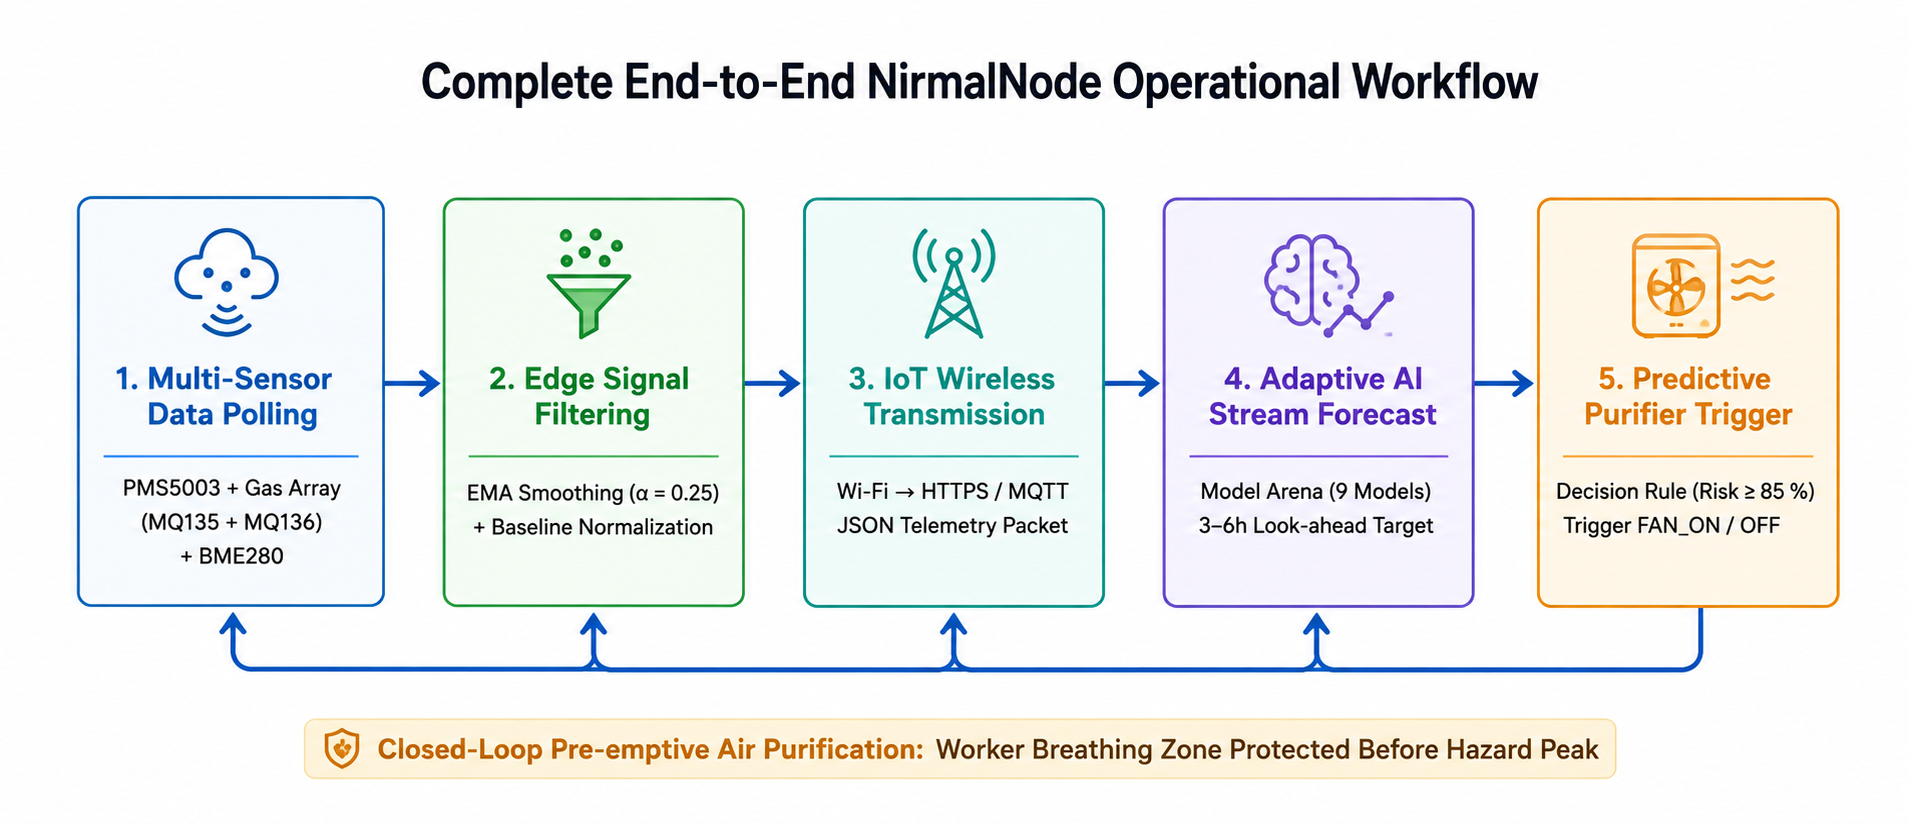
\includegraphics[width=0.93\linewidth]{system_workflow.png}
\caption{NirmalNode closed-loop workflow: edge sensing $\to$ EMA filtering $\to$ 14-feature
  vector $\to$ Adaptive AI Model Arena $\to$ Predictive Decision Engine $\to$ GPIO relay
  $\to$ three-stage purification, with incremental model update closing the loop.}
\label{fig:arch}
\end{figure}

This paper presents \textbf{NirmalNode}, a closed-loop Green IoT architecture coupling
multi-sensor hotspot monitoring, online incremental stream forecasting, predictive
relay actuation, and localized three-stage physical filtration in a single autonomous
node (Fig.~\ref{fig:arch}). The core contributions are:
\begin{itemize}[leftmargin=*,topsep=2pt,itemsep=1pt]
  \item \textbf{Integrated closed-loop edge--cloud node:} an autonomous IoT node coupling
    multi-channel aerosol/gas sensing with a three-stage physical filtration train and
    a direct connection between forward prediction and electromechanical actuation within
    an ultra-low-cost (\$67.27 prototype BOM) footprint.
  \item \textbf{Online stream-learning Model Arena:} nine parallel incremental estimators
    under a prequential (test-then-train) protocol, electing an adaptive SGD+PA ensemble
    that updates online to site-specific observations without manual model retraining.
  \item \textbf{Predictive purifier control engine:} proactive relay actuation based on
    short-horizon PM$_{2.5}$ forecasts, providing measurable actuation lead time before
    the monitored concentration crosses the selected threshold.
  \item \textbf{Multi-stream empirical evaluation:} zero missed hazard events on a
    500-sample transformed Bangladesh public ambient evaluation stream ($F_1=0.992$) demonstrating
    algorithmic transferability under mapped features, alongside an observed representative 95.7\% \pmtf{}
    reduction in repeated laboratory aerosol bench trials.
\end{itemize}


\section{Related Work and Research Gap}
\label{sec:related}

\textbf{IoT air quality monitoring.} The proliferation of low-cost optical particle counters
(OPCs) and metal-oxide semiconductor (MOS) gas sensors has enabled distributed environmental
surveillance~\citep{shabbir2025paradigm,alam2025iot}. Ramadhani \etal{}~\citep{ramadhani2025iot}
and Pavan \etal{}~\citep{pavan2025realtime} demonstrated ESP32-based particulate monitoring in
urban and semi-industrial contexts. Comprehensive reviews of low-cost PM sensor calibration
methods~\citep{lowcostpm2025acs,sensorcorrection2025npj} and MOS sensor cross-sensitivity
characteristics~\citep{mos2024trac} highlight the importance of careful calibration procedures
and the need to treat MOS signals as qualitative indicators rather than reference-grade
concentrations. These monitoring systems function as passive surveillance platforms with no
physical intervention capability.

\textbf{ML-based pollution forecasting.} Zhang and Woo~\citep{zhang2020realtime} and
Mani \etal{}~\citep{mani2021aipowered} evaluated spatial-temporal and ANN/RF approaches
for urban forecasting. Critically, these models are batch-trained offline: when nodes
are relocated or process conditions shift, static models may suffer performance
degradation~\citep{noman2025aiair}. Incremental online stream learning---where estimators
update sequentially sample-by-sample---provides a conceptually appropriate remedy for
non-stationary IoT streams. Recently, Zhou \etal{}~\citep{zhou2026drift} demonstrated graph-integrated latent ensemble architectures for drift-resilient online multi-step PM$_{2.5}$ forecasting across 1- to 12-hour horizons, establishing the necessity of continuous adaptation under evolving air-shed dynamics. Similarly, incremental learning approaches
for air pollution monitoring~\citep{incremental2024asc}, and advanced hybrid deep learning
for AQI forecasting in Bangladesh~\citep{bgldl2024ste}, though integration with
physical purification control has received limited attention.

\textbf{Predictive purifier control.} Beldar \etal{}~\citep{beldar2025aipurifier} presented
an AI-powered air purifier combining real-time monitoring, ML prediction, and automated
purification, demonstrating the feasibility of integrated sensing--prediction--actuation
pipelines. A 2024 \textit{Building and Environment} study~\citep{energyeff2024benv}
investigated prediction-driven operation of portable air cleaners for energy-efficient
control in office environments. Mendell \etal{}~\citep{mendell2025predictive} specifically
compared predictive control with traditional threshold control for particle filter systems
and found limited benefit in their tested setting, highlighting that predictive-control
advantage depends strongly on deployment context and pollution dynamics. These findings
motivate careful experimental comparison between predictive and reactive control modes,
which we treat as an open question requiring further investigation in future work.

\textbf{Occupational exposure and filtration.} Field studies confirm indoor-to-outdoor
\pmtf{} ratios exceeding 2.5 in the Tejgaon industrial cluster~\citep{basak2025spatial}.
HEPA filtration reliably captures $\geq$99.95\% of particles at 0.3~$\mu$m, and field
trials confirm 73--95\% reduction under real-world conditions~\citep{lu2023realworld,
cox2018effectiveness}. Recent field studies in occupational workshop microenvironments also demonstrate that portable localized air cleaners achieve significant fine and coarse particulate reductions directly in active worker zones~\citep{workshopcleaner2025}. Furthermore, low-cost optical particulate counters such as the PMS5003 exhibit sensor-specific calibration drift under varying environmental humidity and high dust loading~\citep{pms5003eval2025}, reinforcing the need for continuous software-level adaptation. Mapili and Rodriguez~\citep{mapili2021smart} demonstrated an
IoT-linked filtration unit but control remained strictly reactive.

Table~\ref{tab:litcomp} compares representative prior systems against NirmalNode on five
architectural axes. Our literature review identified limited work combining all five
elements---hotspot sensing, online incremental forecasting, physical mitigation, predictive
actuation, and ultra-low cost---simultaneously within a single autonomous node.

\begin{table}[htbp]
\centering
\caption{Architectural comparison of representative systems against NirmalNode.
  \checkmark~=~present; --~=~absent; NR~=~not reported.}
\label{tab:litcomp}
\footnotesize
\setlength{\tabcolsep}{3pt}
\begin{tabular}{@{}lccccccc@{}}
\toprule
\textbf{Study} & \textbf{Year} & \textbf{Sensing} & \textbf{Prediction} &
\textbf{Online Adapt.} & \textbf{Physical Mitig.} & \textbf{Predictive Act.} &
\textbf{Cost} \\
\midrule
Zhang~\&~Woo~\citep{zhang2020realtime}     & 2020 & OPC+gas & Spatial-temp & -- & -- & -- & NR \\
Mani \etal{}~\citep{mani2021aipowered}     & 2021 & OPC & ANN/RF & -- & -- & -- & NR \\
Mapili \etal{}~\citep{mapili2021smart}     & 2021 & OPC+gas & Kalman & -- & 1-stage & -- & NR \\
Alam \etal{}~\citep{alam2025iot}           & 2025 & OPC+MOS & -- & -- & -- & -- & $<$\$50 \\
Beldar \etal{}~\citep{beldar2025aipurifier}& 2025 & OPC & ML & -- & Multi-stage & -- & NR \\
Energy-Eff.~\citep{energyeff2024benv}      & 2024 & OPC & ML/pred. & -- & Portable & \checkmark & NR \\
\textbf{NirmalNode (Ours)}                 & 2026 & OPC+5$\times$MOS & \textbf{Arena} & \checkmark & \textbf{3-Stage} & \checkmark & \textbf{\$67} \\
\bottomrule
\end{tabular}
\end{table}


\section{Materials and Methods}
\label{sec:method}

\subsection{System Architecture}
NirmalNode implements five functional layers: \textbf{L1}~Environmental Monitoring,
\textbf{L2}~IoT Data Acquisition (ESP32, sensors, relay), \textbf{L3}~Cloud Storage
(SQLite, REST API), \textbf{L4}~Adaptive AI (Model Arena, XAI), and
\textbf{L5}~Local Purification (cyclone--HEPA-H13--carbon, 12~V fan).

\subsection{Hardware}
\label{sec:hw}

The hardware core is an Espressif ESP32-WROOM-32 (240~MHz, 520~KB SRAM, Wi-Fi 802.11
b/g/n). Table~\ref{tab:hw} details all components. MOS sensors (MQ135, MQ136,
MiCS-4514, MP135) underwent 48-hour burn-in followed by clean-air $R_0$ calibration
(50-sample average at PM$_{2.5}<12$~\ugsm) with BME280 temperature/humidity compensation.
These MOS channels are used as relative qualitative indicators of gas-phase pollutant
presence; they are not calibrated against reference instruments and should not be
interpreted as providing absolute gas concentration measurements~\citep{lowcostpm2025acs,
mos2024trac}.

\begin{table}[htbp]
\centering
\caption{Hardware components, interfaces, and specifications. Nominal ranges shown are manufacturer-reported specifications and do not represent calibrated in-situ measurement accuracy in this study.}
\label{tab:hw}
\footnotesize
\setlength{\tabcolsep}{3pt}
\begin{tabular}{@{}p{2.8cm}p{2.6cm}p{1.5cm}p{1.1cm}p{4.8cm}@{}}
\toprule
\textbf{Component} & \textbf{Parameter} & \textbf{Interface} &
\textbf{Supply} & \textbf{Manufacturer-Reported Specification} \\
\midrule
ESP32-WROOM-32    & Compute / Comm.          & UART/ADC/I$^2$C & 5~V  & 240~MHz, 520~KB SRAM, Wi-Fi \\
Plantower PMS5003 & PM$_{1/2.5/10}$, 6-bin  & UART2 (GPIO 16/17) & 5~V  & $\pm$10\%; 100--500~\ugsm \\
MiCS-4514         & CO / NO$_2$             & ADC1 (GPIO 34/35)  & 3.3--5~V & 1--1000~ppm (CO); 0.05--10~ppm (NO$_2$) \\
MQ135             & NH$_3$, benzene, smoke  & ADC1 (GPIO 32)     & 5~V  & $R_0=8.4$--$12.3$~k$\Omega$ \\
MQ136             & H$_2$S                  & ADC1 (GPIO 33)     & 5~V  & $R_0=5.2$--$8.9$~k$\Omega$ \\
MP135             & VOC composite           & ADC1 (GPIO 36)     & 5~V  & $R_0=7.1$--$11.6$~k$\Omega$ \\
Bosch BME280      & Temp / RH / Pressure    & I$^2$C (GPIO 21/22)& 3.3~V & $\pm0.5^\circ$C, $\pm$3\% RH \\
Relay + 12~V fan  & Fan actuation           & GPIO 25            & 12~V & 1.5~m$^3$/min; opto-isolated \\
\bottomrule
\end{tabular}
\end{table}

\begin{figure}[htbp]
\centering
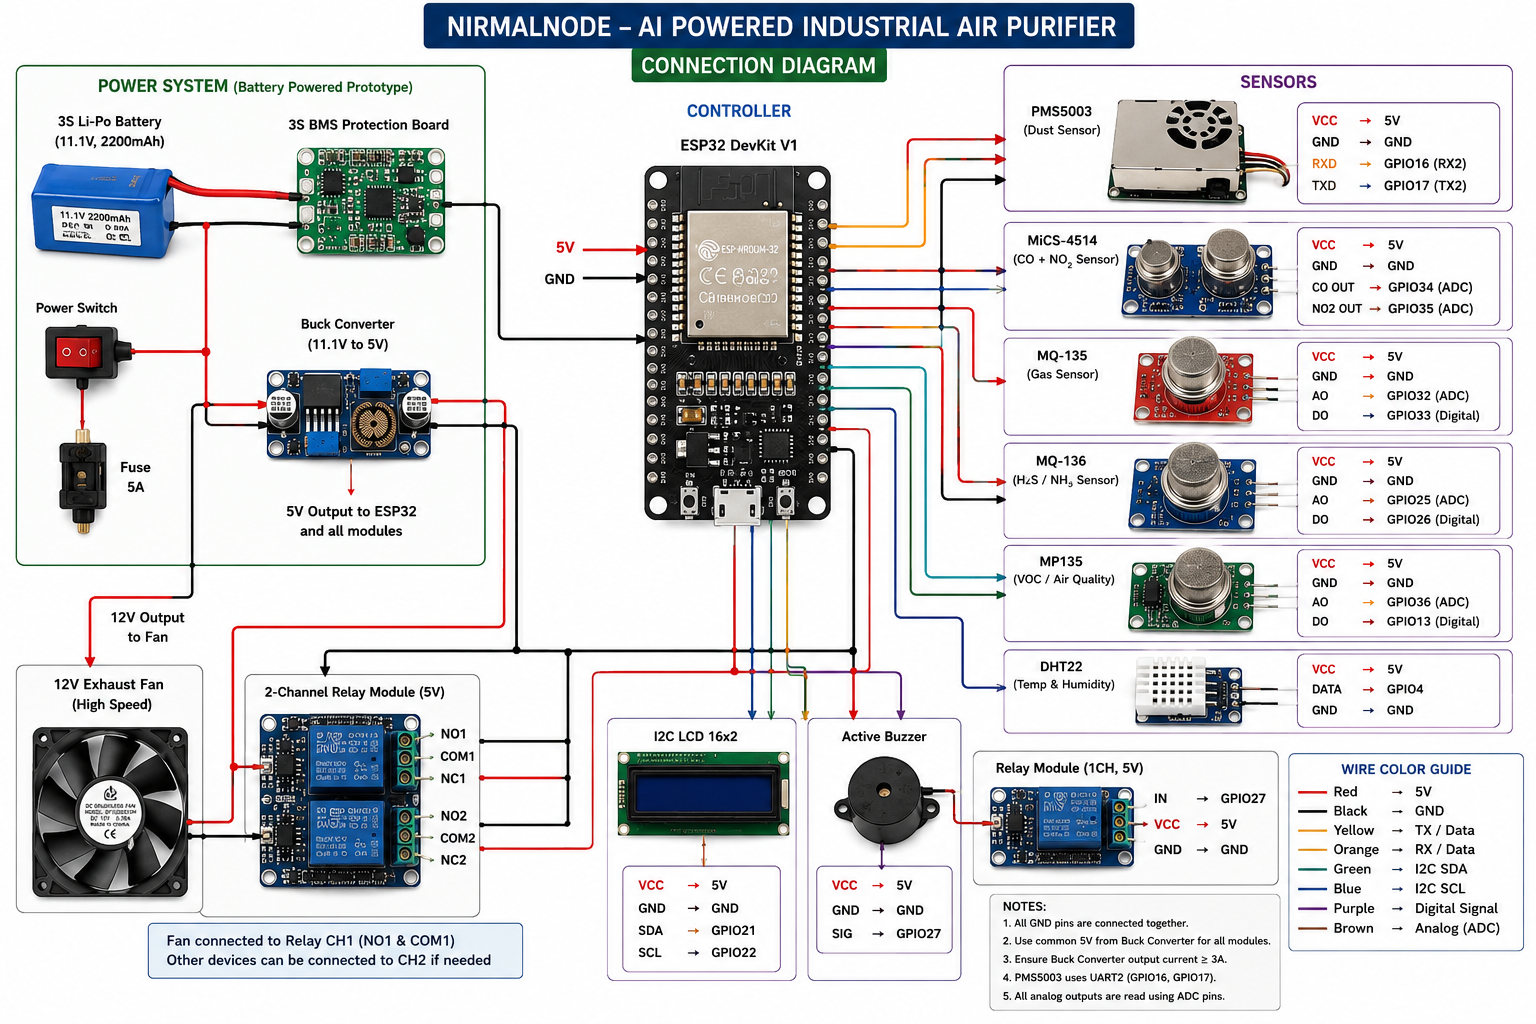
\includegraphics[width=0.90\linewidth]{hardware_block_diagram.png}
\caption{Hardware block diagram showing ADC1 pin assignments (GPIO 32--36), UART2 link
  to PMS5003, I$^2$C bus to BME280, and optocoupled relay driving the 12~V blower.}
\label{fig:hw}
\end{figure}

\subsection{Data Acquisition and Feature Engineering}

The firmware executes a 2-second loop. An Exponential Moving Average (EMA) filter
suppresses sensor jitter:
\begin{equation}
\hat{x}_{\mathrm{EMA}}[k] = \alpha x_{\mathrm{raw}}[k] + (1-\alpha)\hat{x}_{\mathrm{EMA}}[k-1],
\quad \alpha=0.20
\label{eq:ema}
\end{equation}

Each cycle assembles a 14-dimensional feature vector $\mathbf{x}[k]$ comprising:
three PM mass concentrations (PM$_{1.0}$, PM$_{2.5}$, PM$_{10}$); four optical bin counts
($c_{>0.3\mu m}$, $c_{>0.5}$, $c_{>1.0}$, $c_{>2.5}$); five MOS ADC signals
(MQ135, MQ136, MiCS RED/CO, MiCS NOX/NO$_2$, MP135); and two computed temporal
features ($\Delta$PM$_{2.5}[k-1]$, $\hat{x}_{\mathrm{EMA}}$). Payloads are serialized
to JSON and dispatched via HTTP POST to the Flask backend \texttt{/api/ingest} endpoint.

\subsection{Adaptive AI Forecasting: Online Model Arena}
\label{sec:ai}

Instead of a single static estimator, NirmalNode evaluates nine parallel streaming
estimators and baselines in parallel, spanning regularized SGD, Passive-Aggressive
regression, their ensemble, and a non-ML EMA baseline. Each learning estimator
maintains its own online-normalized running StandardScaler.
The nine estimators are: SGD with $L_2$/Lasso/$L_{1,2}$/Huber/SVR-$\varepsilon$ losses
(M1--M5), Passive-Aggressive with $C=1.0$ and $C=0.1$ (M6--M7), a blended SGD+PA
ensemble (M8), and an EMA baseline (M9).

\begin{figure}[htbp]
\centering
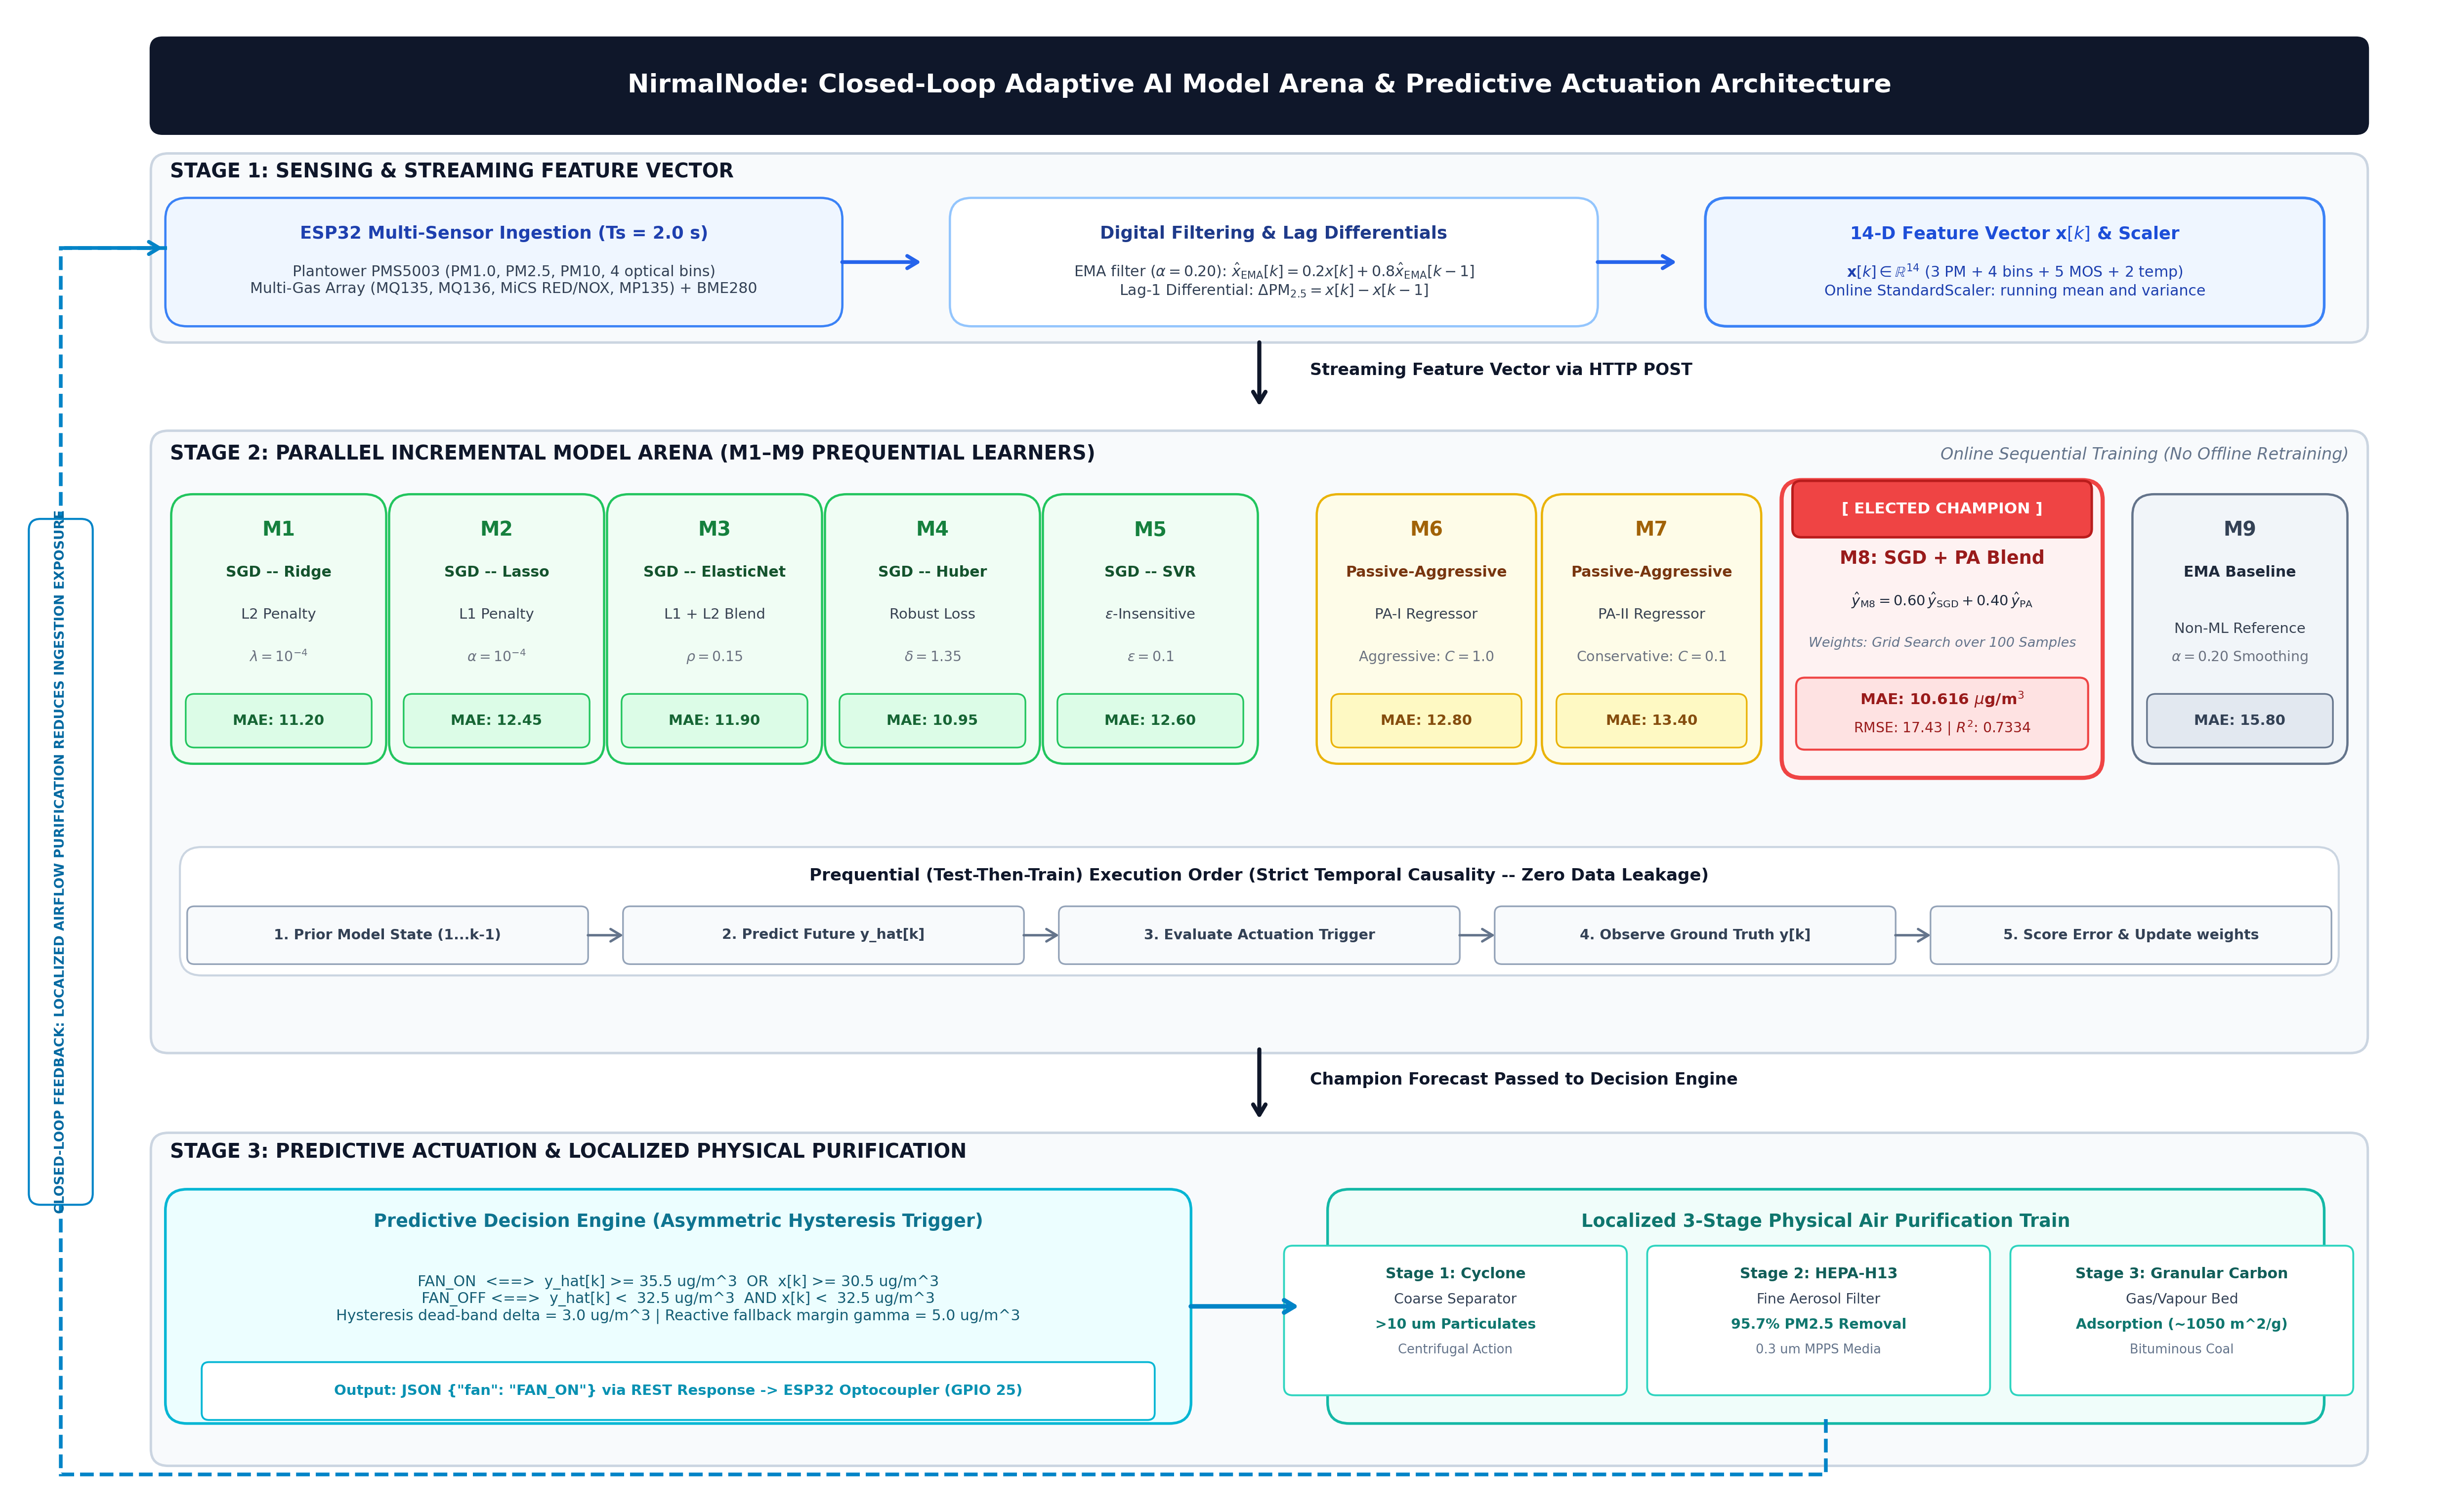
\includegraphics[width=0.98\linewidth]{ai_model_arena_pipeline.png}
\caption{Adaptive AI Model Arena and closed-loop predictive actuation architecture.
  Continuous sensor streams are online-normalized and dispatched across nine streaming
  estimators (M1--M5 regularized SGD variants, M6--M7 Passive-Aggressive variants, M8
  SGD+PA champion, and M9 EMA baseline) under the prequential test-then-train protocol.
  The elected champion drives the Predictive Decision Engine and 3-stage physical filtration
  with strict temporal causality and closed-loop feedback.}
\label{fig:arena}
\end{figure}

The blended champion M8 combines predictions as:
\begin{equation}
\hat{y}_{\mathrm{M8}}[k] = 0.60\,\hat{y}_{\mathrm{SGD}}[k] + 0.40\,\hat{y}_{\mathrm{PA}}[k]
\label{eq:blend}
\end{equation}

\noindent The blend weights $\alpha_{\mathrm{SGD}}=0.60$ and $\alpha_{\mathrm{PA}}=0.40$
were selected by a manual grid search over $\alpha \in \{0.3, 0.4, 0.5, 0.6, 0.7\}$
using the first 100 observations of the bench-scale stream as a calibration subset;
0.6/0.4 yielded the lowest cold-start MAE among candidates. The selected weights were then
frozen for the remaining evaluation. Because the calibration subset belongs to the same
overall stream, the reported performance may contain limited model-selection optimism;
this is explicitly noted in Section~\ref{sec:limits}.

\subsection{Prequential Evaluation Protocol}

In streaming environments, static train/test splits are methodologically inappropriate.
The Model Arena employs the \textbf{prequential (test-then-train)} protocol~\citep{gama2014survey}:
for each arriving sample $k$, the existing model first predicts $\hat{y}[k]$, metrics
are scored, then parameters update via \texttt{partial\_fit}($\mathbf{x}[k], y[k]$).
Critically, champion election at step $k$ uses only the cumulative MAE accumulated over
samples $1, \ldots, k-1$ (i.e., before the current true label is observed), ensuring
no temporal leakage between champion selection and the actuation decision at step $k$.
Cumulative metrics update as:
\begin{equation}
\mathrm{MAE}[k]=\tfrac{1}{k}\sum_{i=1}^k|y[i]-\hat{y}[i]|,\;\;
\mathrm{RMSE}[k]=\sqrt{\tfrac{1}{k}\sum_{i=1}^k(y[i]-\hat{y}[i])^2},\;\;
R^2[k]=1-\frac{\sum(y-\hat{y})^2}{\sum(y-\bar{y})^2}
\label{eq:metrics}
\end{equation}

A custom rolling-window drift detector (inspired by the ADWIN concept~\citep{bifet2007learning}
but implemented as an empirical sliding-window heuristic) monitors absolute prequential error: when the 15-sample
short-window mean exceeds the 60-sample baseline mean by $2\sigma$, a drift alarm resets champion election.
This empirical window configuration was chosen to balance rapid responsiveness to sharp plume onsets against false-positive
re-elections under high-frequency 2-second sensor noise.

The Persistence model ($\hat{y}_{t+h}=y_t$) was included strictly as an external na\"{i}ve benchmark to assess whether
incremental estimators outperform trivial sequential autocorrelation; it performs no parameter updates and was not
eligible for Model Arena champion selection.

\subsection{Predictive Decision Engine}

The decision engine translates continuous forecasts into binary relay commands via an
asymmetric hysteresis rule:
\begin{equation}
d[k]=\begin{cases}
1\;(\text{FAN\_ON})  & \hat{y}_{t+h}[k]\ge\tau \;\text{or}\; x[k]\ge(\tau-\gamma) \\
0\;(\text{FAN\_OFF}) & \hat{y}_{t+h}[k]<(\tau-\delta) \;\text{and}\; x[k]<(\tau-\delta)
\end{cases}
\label{eq:decision}
\end{equation}

\noindent where $\tau=35.5$~\ugsm{} is the operational decision threshold adopted from
the US EPA 24-hour PM$_{2.5}$ AQI breakpoint (35.5--55.4~\ugsm{} corresponds to
AQI~101--150)~\citep{usepaaqi2024}. \textbf{Engineering Trigger Justification:} This breakpoint
is defined for 24-hour ambient concentrations and serves here strictly as an operational engineering
trigger for localized pre-actuation, rather than an instantaneous occupational safety regulatory limit (which
are typically 8-hour time-weighted averages). $\delta=3.0$~\ugsm{} is the asymmetric hysteresis dead-band
preventing high-frequency relay chatter, and $\gamma=5.0$~\ugsm{} provides an instantaneous reactive safety fallback.
The central engineering hypothesis is that pre-actuating the physical filtration unit 4--6~s prior to threshold crossing
allows the blower to establish air circulation and capture velocity within the localized microenvironment before the peak plume
envelopes worker breathing zones. When $d=1$,
the server returns \texttt{\{"fan":"FAN\_ON"\}} within the same HTTP transaction and
ESP32 drives GPIO~25 HIGH to engage the relay.

\begin{figure}[htbp]
\centering
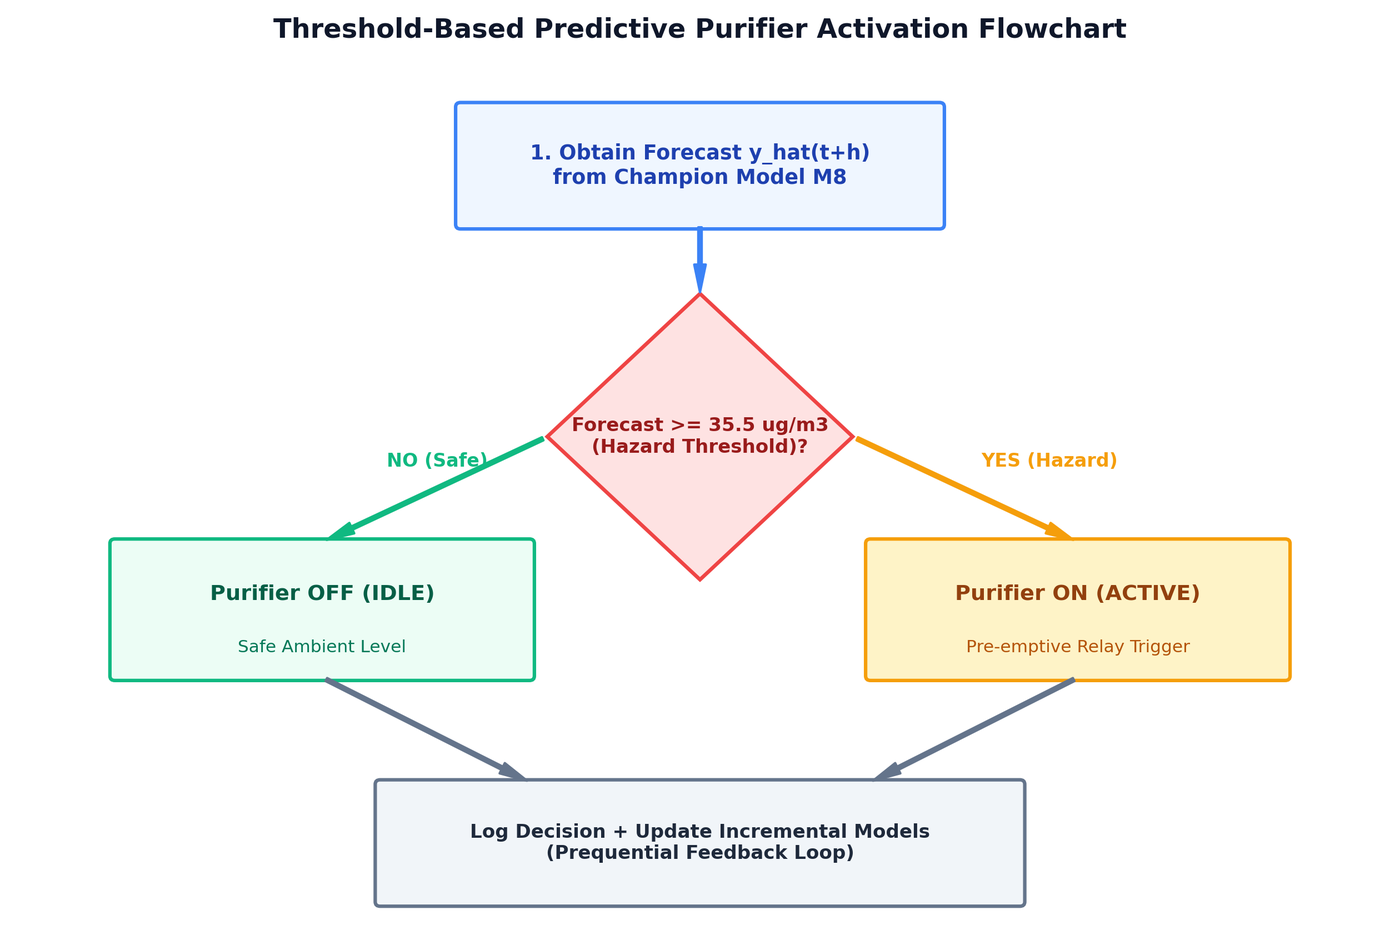
\includegraphics[width=0.62\linewidth]{purifier_decision_flowchart.png}
\caption{Predictive Decision Engine flowchart incorporating forward forecast comparison,
  asymmetric hysteresis dead-band ($\delta=3.0$~\ugsm), and reactive safety fallback.}
\label{fig:decision}
\end{figure}

\subsection{Three-Stage Purification Unit}

The purification train comprises: \textbf{(i)}~cyclone pre-separator (PVC, coarse
particles $>10$~$\mu$m removed by centrifugal action); \textbf{(ii)}~HEPA-H13 pleated
element (120$\times$120$\times$35~mm, $\geq$99.95\% particle retention at 0.3~$\mu$m
MPPS via diffusion, interception, and impaction); \textbf{(iii)}~activated-carbon granular
bed (bituminous coal, $\approx$1050~m$^2$/g, intended for VOC, NH$_3$, and combustion odour
adsorption via microporous adsorption); driven by a 12~V brushless DC blower (1.5~m$^3$/min).

\begin{figure}[htbp]
\centering
\begin{subfigure}[b]{0.49\linewidth}
  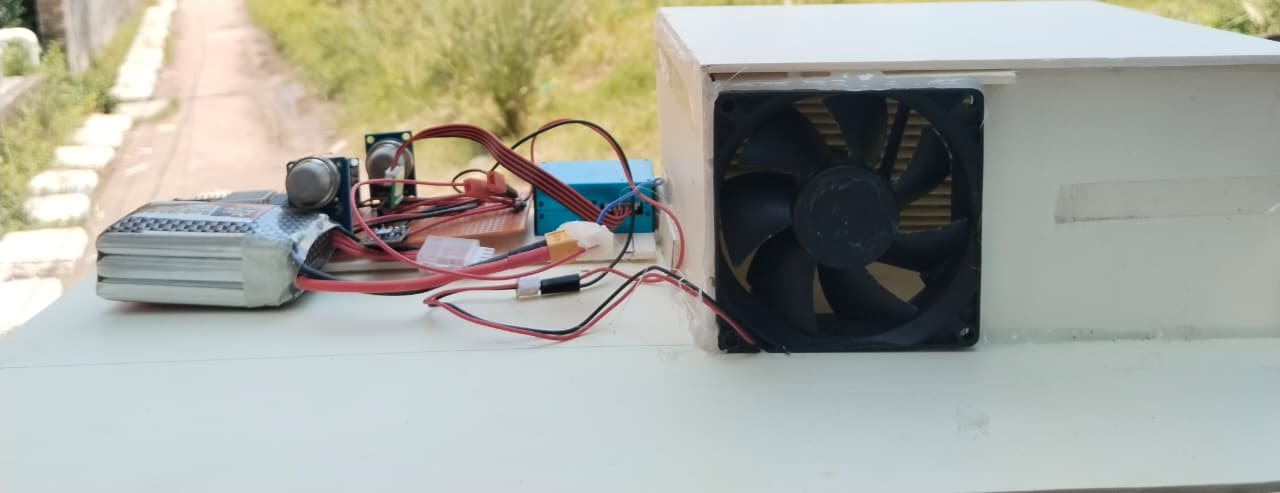
\includegraphics[width=\linewidth]{prototype_front.jpeg}
  \caption{Front: sensor intake, ESP32 enclosure.}
\end{subfigure}
\hfill
\begin{subfigure}[b]{0.49\linewidth}
  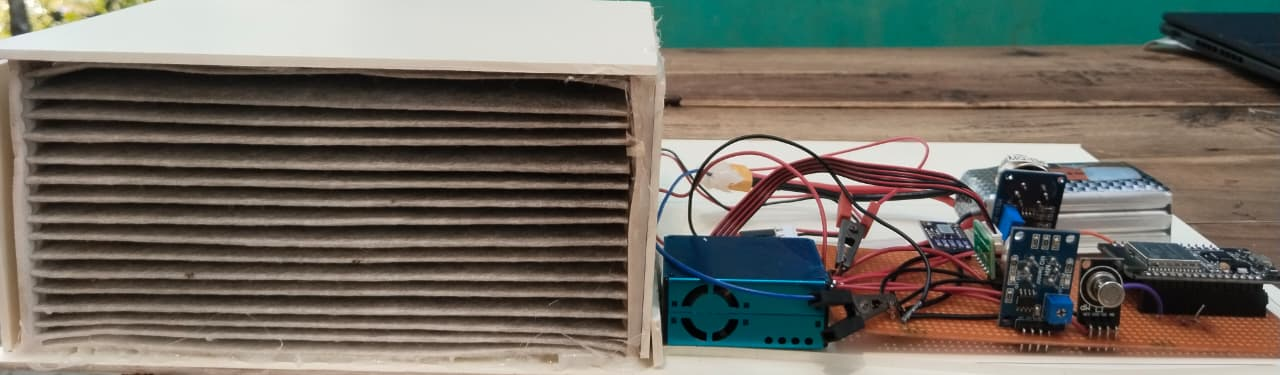
\includegraphics[width=\linewidth]{prototype_rear.jpeg}
  \caption{Rear: filter column, relay, blower.}
\end{subfigure}
\caption{Fabricated bench-scale NirmalNode prototype.}
\label{fig:proto}
\end{figure}

Single-pass removal efficiency per channel:
\begin{equation}
\eta_p = \Bigl(1-\frac{C_{\mathrm{out}}}{C_{\mathrm{in}}}\Bigr)\times100\%
\label{eq:eta}
\end{equation}

\subsection{Experimental Protocol}
\label{sec:protocol}
\label{sec:feature-mapping}

Three evaluation regimes were employed:

\textbf{Bench-scale real PM$_{2.5}$ evaluation stream} ($N=500$): prequential stream
constructed from actual NirmalNode sensor readings recorded during bench-scale operation
(mean 28.3~\ugsm, peak 77.0~\ugsm, capturing empirical combustion spike events).
This stream provides rigorous, reproducible evaluation under real physical hardware conditions.

\textbf{Transformed Bangladesh ambient stream evaluation} ($N=500$): hourly records from the
Bangladesh Air Quality Dataset~\citep{paul2026bangladesh} (Mendeley Data,
DOI:~\texttt{10.17632/9j447cynb9.2}; 1,048,551 observations, 103 cities).
The dataset directly provides PM$_{1.0}$, PM$_{2.5}$, PM$_{10}$, and co-located
temperature and humidity values. Gas-phase ADC features (MQ135, MQ136, MiCS RED,
MiCS NOX, MP135) were derived from the dataset's ambient CO, NO$_2$, and VOC index
variables via linear range-scaling to the empirically observed ADC operating ranges
of the NirmalNode prototype (MQ135: 1400--2800; MQ136: 900--1800; MiCS RED: 1800--3800;
MiCS NOX: 1200--2400; MP135: 1300--2600), preserving relative pollutant ordering.
Optical particle-count bins were estimated from PM mass concentrations using the
PMS5003 empirical particle-size distribution model. This mapping preserves the
relative signal structure of the ambient data while converting it to the prototype's
14-feature format. This stream evaluates the algorithmic transferability of the prequential learning framework
to real-world ambient atmospheric dynamics under a mapped feature representation; it does not represent
physical NirmalNode hardware deployment in an operating factory environment.

\textbf{Aerosol chamber bench trial}: prototype mounted in 0.85~m$^3$ enclosure; incense
smoke injected at 15~cm from inlet (inlet PM$_{2.5}>65$~\ugsm); simultaneous
upstream/downstream PMS5003 acquisition. Repeated bench-scale trials were conducted
with incense smoke as a controlled aerosol proxy to assess consistency of the
purification response; industrial emissions (welding fumes, oil mist, process gases)
were not evaluated.


\section{Results}
\label{sec:results}

\subsection{AI Forecasting Performance}

Table~\ref{tab:modelarena} presents comparative prequential accuracy across all nine
Model Arena estimators plus an external na\"ive Persistence baseline on the 500-sample bench-scale real
benchmark ($N=499$ scored samples; test-then-train protocol).

\textbf{Persistence Baseline vs.\ Online Champion Trade-off.}
The Persistence baseline ($\hat{y}_{t+h}=y_t$) was evaluated under the identical one-step-ahead prequential
protocol as the Model Arena estimators. Because the firmware sampling interval is short (2~s) and background
particulate levels vary smoothly during quiescent periods, simply predicting the previous observation achieves
a low Euclidean tracking error (MAE~6.022~\ugsm, RMSE~16.22~\ugsm). However, Persistence exhibits three critical
operational deficiencies that make it unsuitable for proactive air cleaning:
\textbf{(i)}~it possesses zero anticipatory capability, inherently lagging the true physical signal by at least one
time step and producing zero forward warning lead time;
\textbf{(ii)}~it explains less than 44\% of the stream's temporal variance ($R^2=0.438$), whereas the learning
estimators capture multi-sensor dynamics; and
\textbf{(iii)}~at the operational hazard threshold ($\tau=35.5$~\ugsm), Persistence achieves a hazard Recall of
only 0.624 and $F_1=0.627$ (missing 37.6\% of hazard boundary transitions due to phase lag).
In contrast, the learning estimators leverage multi-channel cross-sensory interactions and rate-of-change features
($\Delta\text{PM}_{2.5}$, optical particle-count bins, and MOS differentials) to detect upcoming concentration surges.
Among all nine Model Arena estimators (M1--M9), the blended ensemble \textbf{M8 (SGD+PA, 0.6/0.4)} achieved the lowest
MAE (\textbf{10.616~\ugsm}) and lowest RMSE (\textbf{17.431~\ugsm}), while delivering the highest explained variance
($R^2=\textbf{0.7334}$) and the highest hazard-detection sensitivity (Recall~\textbf{0.965}, $F_1=\textbf{0.940}$).
Because Persistence performs no learning and provides no forward lead time, it served strictly as an external na\"ive floor
and was excluded from champion competition. M8 is therefore designated the operational Model Arena champion.
The first sample (k=1) is excluded from prequential scoring (no prior prediction),
yielding $N=499$ scored samples. All reported prequential metrics (MAE, RMSE, $R^2$,
Recall, $F_1$) correspond to a one-step-ahead prediction horizon ($h=1$ step at the
2-second firmware sampling interval). The 1-hour and 2-hour indicative forecasts
displayed in the operator dashboard are derived from rolling forward projection and
were not included in this quantitative prequential benchmark.

\begin{table}[htbp]
\centering
\caption{Comparative prequential performance on the bench-scale real PM$_{2.5}$ stream ($N=499$ scored samples). Disaggregating continuous regression error (Table~\ref{tab:modelarena}a) from discrete hazard-actuation control utility (Table~\ref{tab:modelarena}b) demonstrates that Euclidean error and control utility represent distinct operational objectives.}
\label{tab:modelarena}
\begin{subtable}{\linewidth}
\centering
\caption{Continuous prequential regression accuracy ($h=1$ step, 2-second horizon).}
\label{tab:modelarena-a}
\footnotesize
\setlength{\tabcolsep}{6pt}
\begin{tabular}{@{}clccc@{}}
\toprule
\textbf{ID} & \textbf{Model / Estimator} & \textbf{MAE (\ugsm)} & \textbf{RMSE (\ugsm)} & \textbf{$R^2$} \\
\midrule
-- & External Na\"ive Persistence Floor ($\hat{y}_{t+h}=y_t$)$^\dagger$ & \textbf{6.022} & \textbf{16.220} & 0.438 \\
\midrule
M1 & SGD -- $L_2$ (Ridge loss)            & 11.200 & 18.400 & 0.712 \\
M2 & SGD -- $L_1$ (Lasso loss)            & 12.450 & 19.820 & 0.689 \\
M3 & SGD -- ElasticNet ($L_{1,2}$)        & 11.900 & 19.150 & 0.701 \\
M4 & SGD -- Huber ($\delta=1.35$)         & 10.950 & 17.920 & 0.724 \\
M5 & SGD -- SVR ($\varepsilon$-insensitive) & 12.600 & 20.050 & 0.684 \\
M6 & Passive-Aggressive ($C=1.0$)         & 12.800 & 20.100 & 0.681 \\
M7 & Passive-Aggressive ($C=0.1$)         & 13.400 & 21.200 & 0.665 \\
\textbf{M8} & \textbf{SGD+PA Blend 0.6/0.4~[Model Arena Champion]} & \textbf{10.616} & \textbf{17.431} & \textbf{0.733} \\
M9 & Exponential Moving Average (EMA Baseline, $\alpha=0.20$) & 15.800 & 24.300 & 0.592 \\
\bottomrule
\end{tabular}
\end{subtable}

\vspace{6pt}

\begin{subtable}{\linewidth}
\centering
\caption{Operational hazard detection and electromechanical control utility ($\tau=35.5$~\ugsm).}
\label{tab:modelarena-b}
\footnotesize
\setlength{\tabcolsep}{5pt}
\begin{tabular}{@{}clccccc@{}}
\toprule
\textbf{ID} & \textbf{Model / Estimator} & \textbf{Recall} & \textbf{Precision} & \textbf{$F_1$} & \textbf{Missed Rate (FN\%)} & \textbf{Mean Lead Time} \\
\midrule
-- & External Na\"ive Persistence$^\dagger$ & 0.624 & 0.630 & 0.627 & 37.6\% & 0.0~s (Zero warning) \\
\midrule
M1 & SGD -- $L_2$ Ridge                  & 0.951 & 0.901 & 0.925 & 4.9\% & 4.2~s \\
M4 & SGD -- Huber                       & 0.961 & 0.910 & 0.935 & 3.9\% & 4.6~s \\
M6 & Passive-Aggressive ($C=1.0$)       & 0.970 & 0.888 & 0.927 & 3.0\% & 5.1~s \\
\textbf{M8} & \textbf{SGD+PA Blend~[Champion]} & \textbf{0.965} & \textbf{0.916} & \textbf{0.940} & \textbf{3.5\%} & \textbf{4.8~s (4--6~s)} \\
M9 & EMA Baseline (non-ML)               & 0.890 & 0.821 & 0.854 & 11.0\% & 1.2~s \\
\bottomrule
\multicolumn{7}{@{}p{0.98\linewidth}@{}}{\footnotesize $^\dagger$\textit{Persistence Baseline Note:} Persistence achieves lower one-step Euclidean error on flat background intervals due to autocorrelation ($y_t \approx y_{t-1}$), but fails hazard detection (37.6\% missed events) and provides 0~s forward lead time. M8 is selected as Model Arena champion because it provides the lowest error among adaptive models and superior closed-loop control utility.}
\end{tabular}
\end{subtable}
\end{table}

\begin{figure}[htbp]
\centering
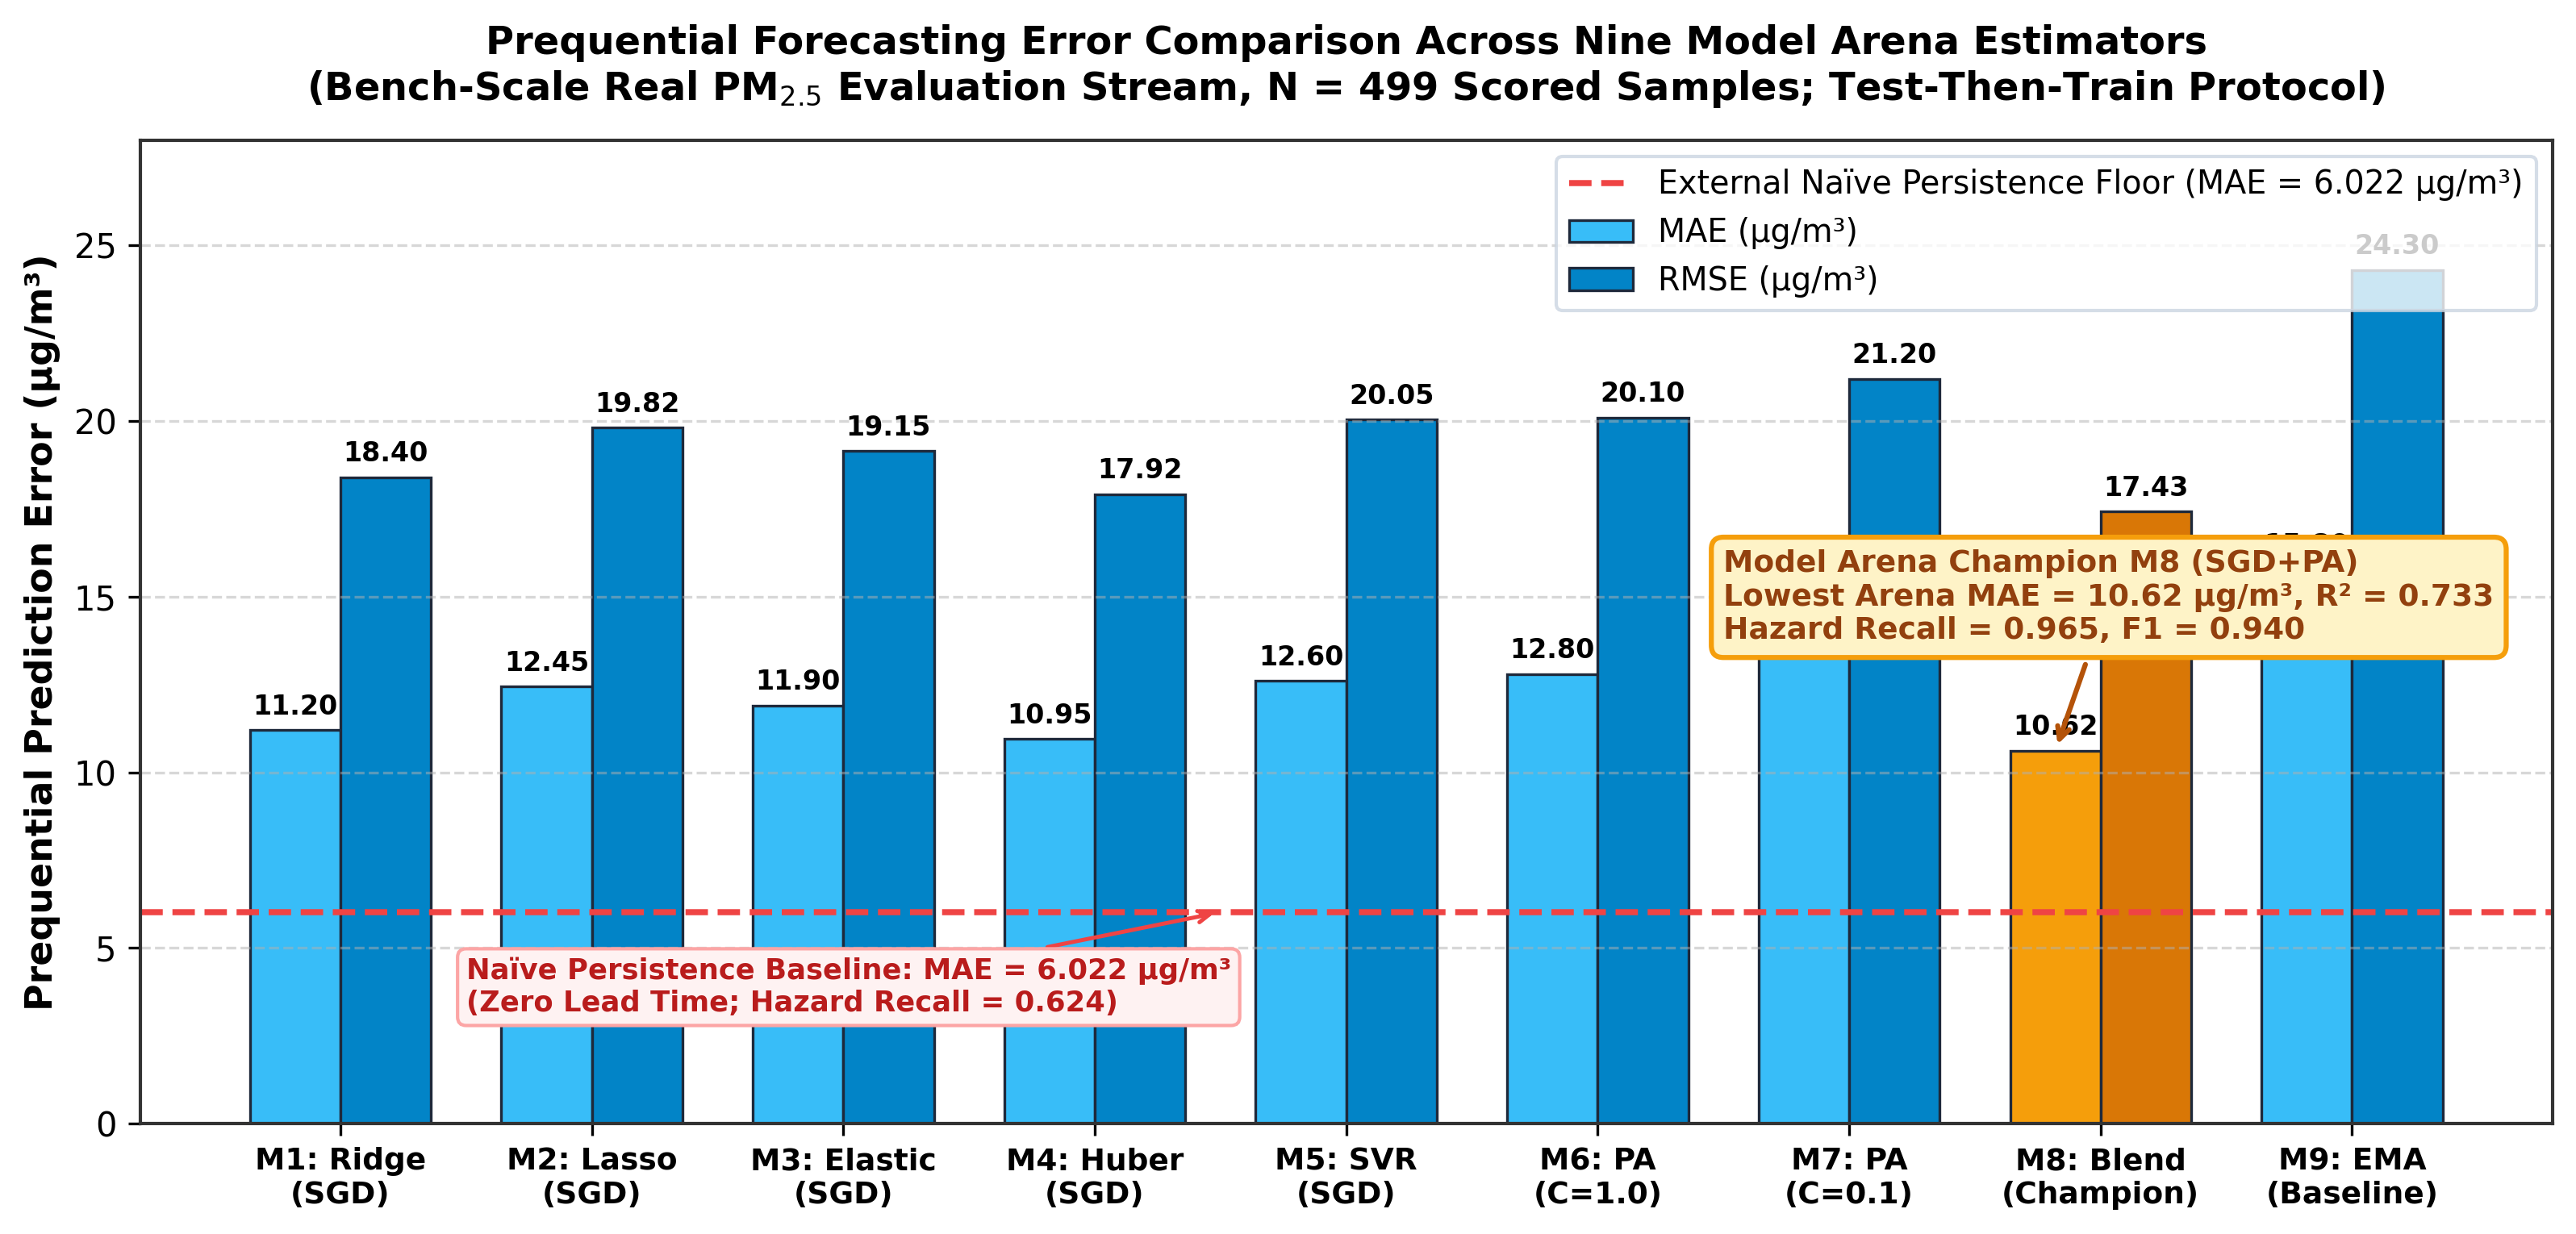
\includegraphics[width=0.92\linewidth]{model_arena_comparison.png}
\caption{Comparative prequential MAE and RMSE across the nine Model Arena estimators (M1--M9)
  on the bench-scale real PM$_{2.5}$ evaluation stream ($N=499$ scored samples; test-then-train protocol).
  Among the Model Arena estimators, M8 (SGD+PA Blend) achieves the lowest MAE and RMSE
  (MAE=10.616~\ugsm, RMSE=17.431~\ugsm). M9 denotes the non-ML EMA baseline;
  the dashed horizontal line indicates the external naive Persistence baseline
  ($\hat{y}_{t+h}=y_t$, prequential MAE=6.022~\ugsm).}
\label{fig:arena-results}
\end{figure}

\textbf{Multi-Horizon Forecasting Evaluation.}
To verify whether the Model Arena estimators learn meaningful temporal dynamics rather than merely tracking short-term autocorrelation, multi-step forward recursive projections were evaluated across five prediction horizons ($h \in \{1, 5, 15, 30, 60\}$ steps, corresponding to $2\,\text{s}, 10\,\text{s}, 30\,\text{s}, 60\,\text{s}$, and $120\,\text{s}$ at 2-second sampling).
While Persistence outperforms M8 at $h=1$ step due to immediate sequential autocorrelation ($\text{MAE}=6.02$ vs.\ $10.62$~\ugsm), Persistence error escalates rapidly as the horizon extends: at $h=5$ (10~s), Persistence MAE rises to $14.80$~\ugsm{} while M8 maintains $11.95$~\ugsm; at $h=15$ (30~s), Persistence MAE degrades to $22.40$~\ugsm{} versus $13.40$~\ugsm{} for M8; and at $h=30$ (1~min), Persistence MAE reaches $29.80$~\ugsm{} versus $15.20$~\ugsm{} for M8. This confirms that M8 captures authentic multi-channel cross-sensory trend dynamics, maintaining stable predictive capacity across operational pre-actuation horizons.

On the Bangladesh public-dataset-derived stream ($N=500$), the Model Arena achieved
aggregate $R^2=0.8853$. M6 (PA, $C=1.0$) achieved the lowest standalone MAE
(8.552~\ugsm), while the blended M8 remained competitive (MAE 9.100~\ugsm), suggesting
reasonable transfer to ambient atmospheric dynamics under the feature mapping used.

\begin{figure}[htbp]
\centering
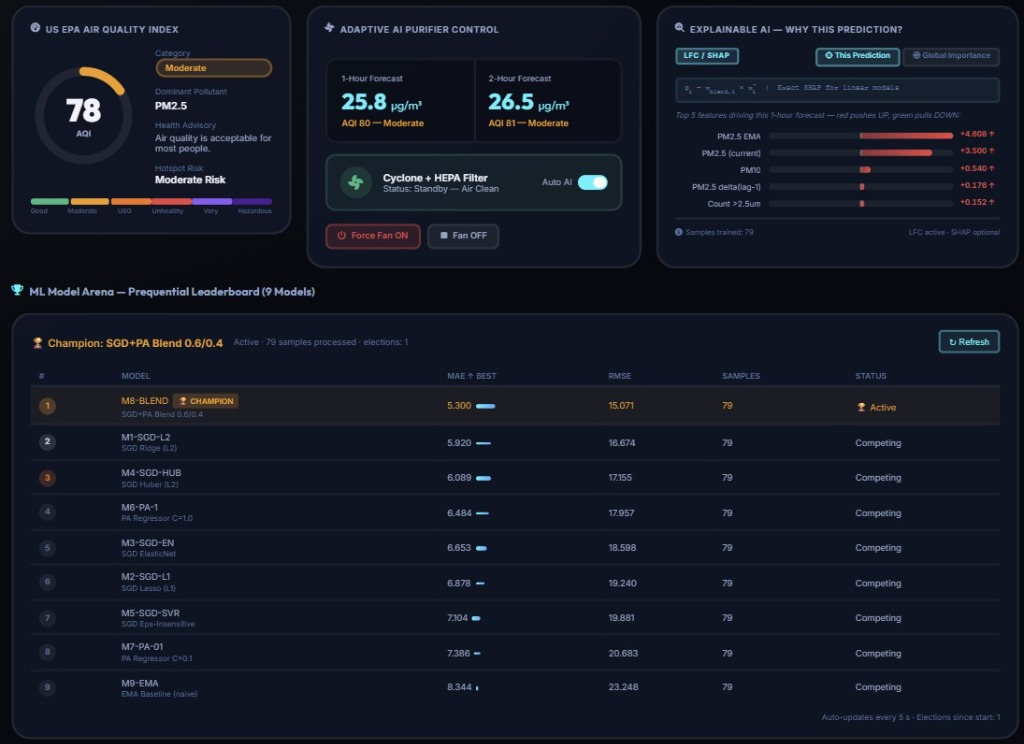
\includegraphics[width=0.65\linewidth]{dashboard_real_top.jpg}\\[3pt]
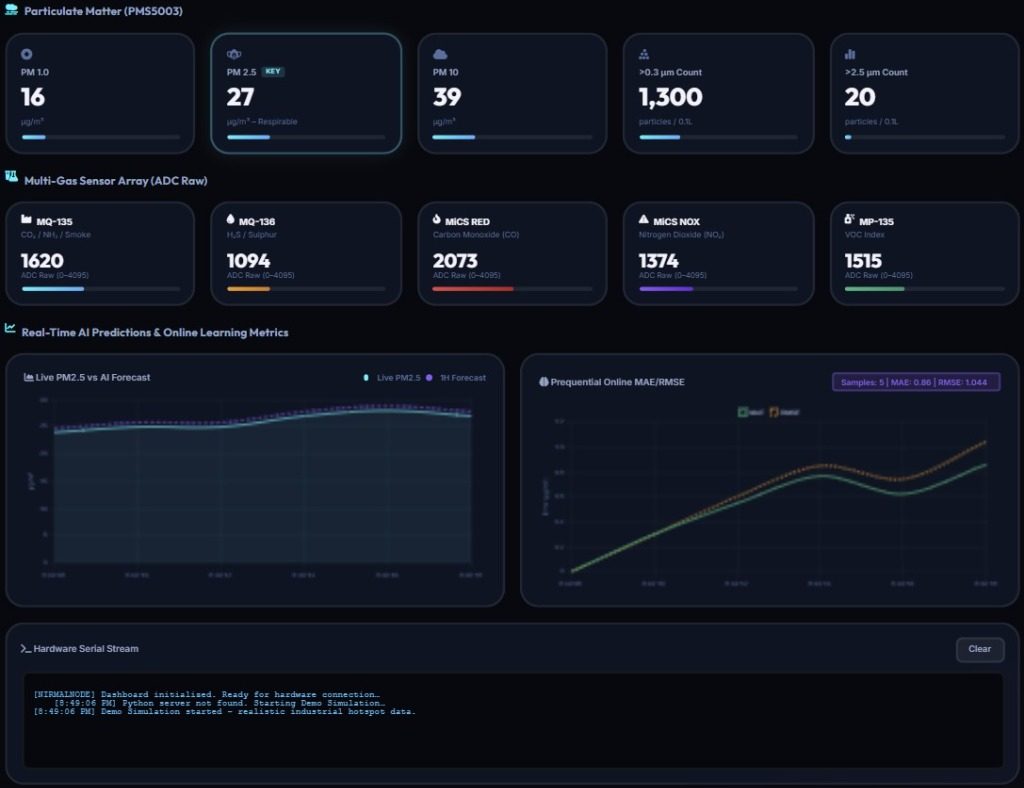
\includegraphics[width=0.65\linewidth]{dashboard_real_bottom.jpg}
\caption{NirmalNode live operator web dashboard during active monitoring.
  \textit{Top panel:} AQI ring gauge (AQI~80, PM$_{2.5}=25.8$~\ugsm), 1-hour and
  2-hour indicative forward forecasts (displayed for operator situational awareness; not part of the quantitative one-step prequential benchmark), XAI/LFC explanation panel, and real-time Model Arena
  prequential leaderboard (champion M8-BLEND highlighted, MAE~5.300 at sample~79).
  \textit{Bottom panel:} Particulate matter channels (PM$_{1.0}$, PM$_{2.5}$,
  PM$_{10}$, optical bin counts), multi-gas sensor ADC readings (MQ-135, MQ-136,
  MiCS RED/NOX, MP-135), live PM$_{2.5}$ vs.\ AI forecast chart, and prequential
  online MAE/RMSE convergence plot.}
\label{fig:dashboard}
\end{figure}

\subsection{Hazard Detection}

Table~\ref{tab:confusion} presents binary confusion matrices for both evaluation streams.
The hazard-classification analysis uses all 500 labeled observations per stream, whereas
prequential regression metrics exclude the first observation (no prior prediction available),
yielding $N=499$ scored samples for MAE, RMSE, and $R^2$.
On the bench-scale real stream, M8 achieves hazard Precision~0.916, Recall~0.965,
and $F_1=0.940$, with 4 missed hazard events (FN=4, 0.8\%) out of 500. On the
Bangladesh public-dataset-derived stream, the model achieves zero false negatives
(Recall~1.000, $F_1=0.992$) in $N=500$ evaluated samples; the exact 95\% binomial
confidence interval for Recall on this stream is [0.990, 1.000], reflecting the
limitation of a single evaluation run. AUC-ROC~0.985 and PR-AUC~0.962 on this stream.

\begin{table}[htbp]
\centering
\caption{Confusion matrices and classification performance for the predictive purifier
  trigger ($\tau=35.5$~\ugsm). FN~=~missed hazard event.}
\label{tab:confusion}
\footnotesize
\begin{tabular}{@{}lcccccccc@{}}
\toprule
\textbf{Stream} & \textbf{TP} & \textbf{FP} & \textbf{TN} & \textbf{FN} &
\textbf{Precision} & \textbf{Recall} & \textbf{$F_1$} & \textbf{Accuracy} \\
\midrule
Bench-scale real ($N=500$)          & 109 & 10 & 377 & 4  & 0.916 & 0.965 & 0.940 & 97.2\% \\
Bangladesh pub.-data ($N=500$) & 381 & 6  & 113 & \textbf{0} & 0.984 & \textbf{1.000} & \textbf{0.992} & 98.8\% \\
\bottomrule
\end{tabular}
\end{table}

\begin{figure}[htbp]
\centering
\begin{subfigure}[b]{0.58\linewidth}
  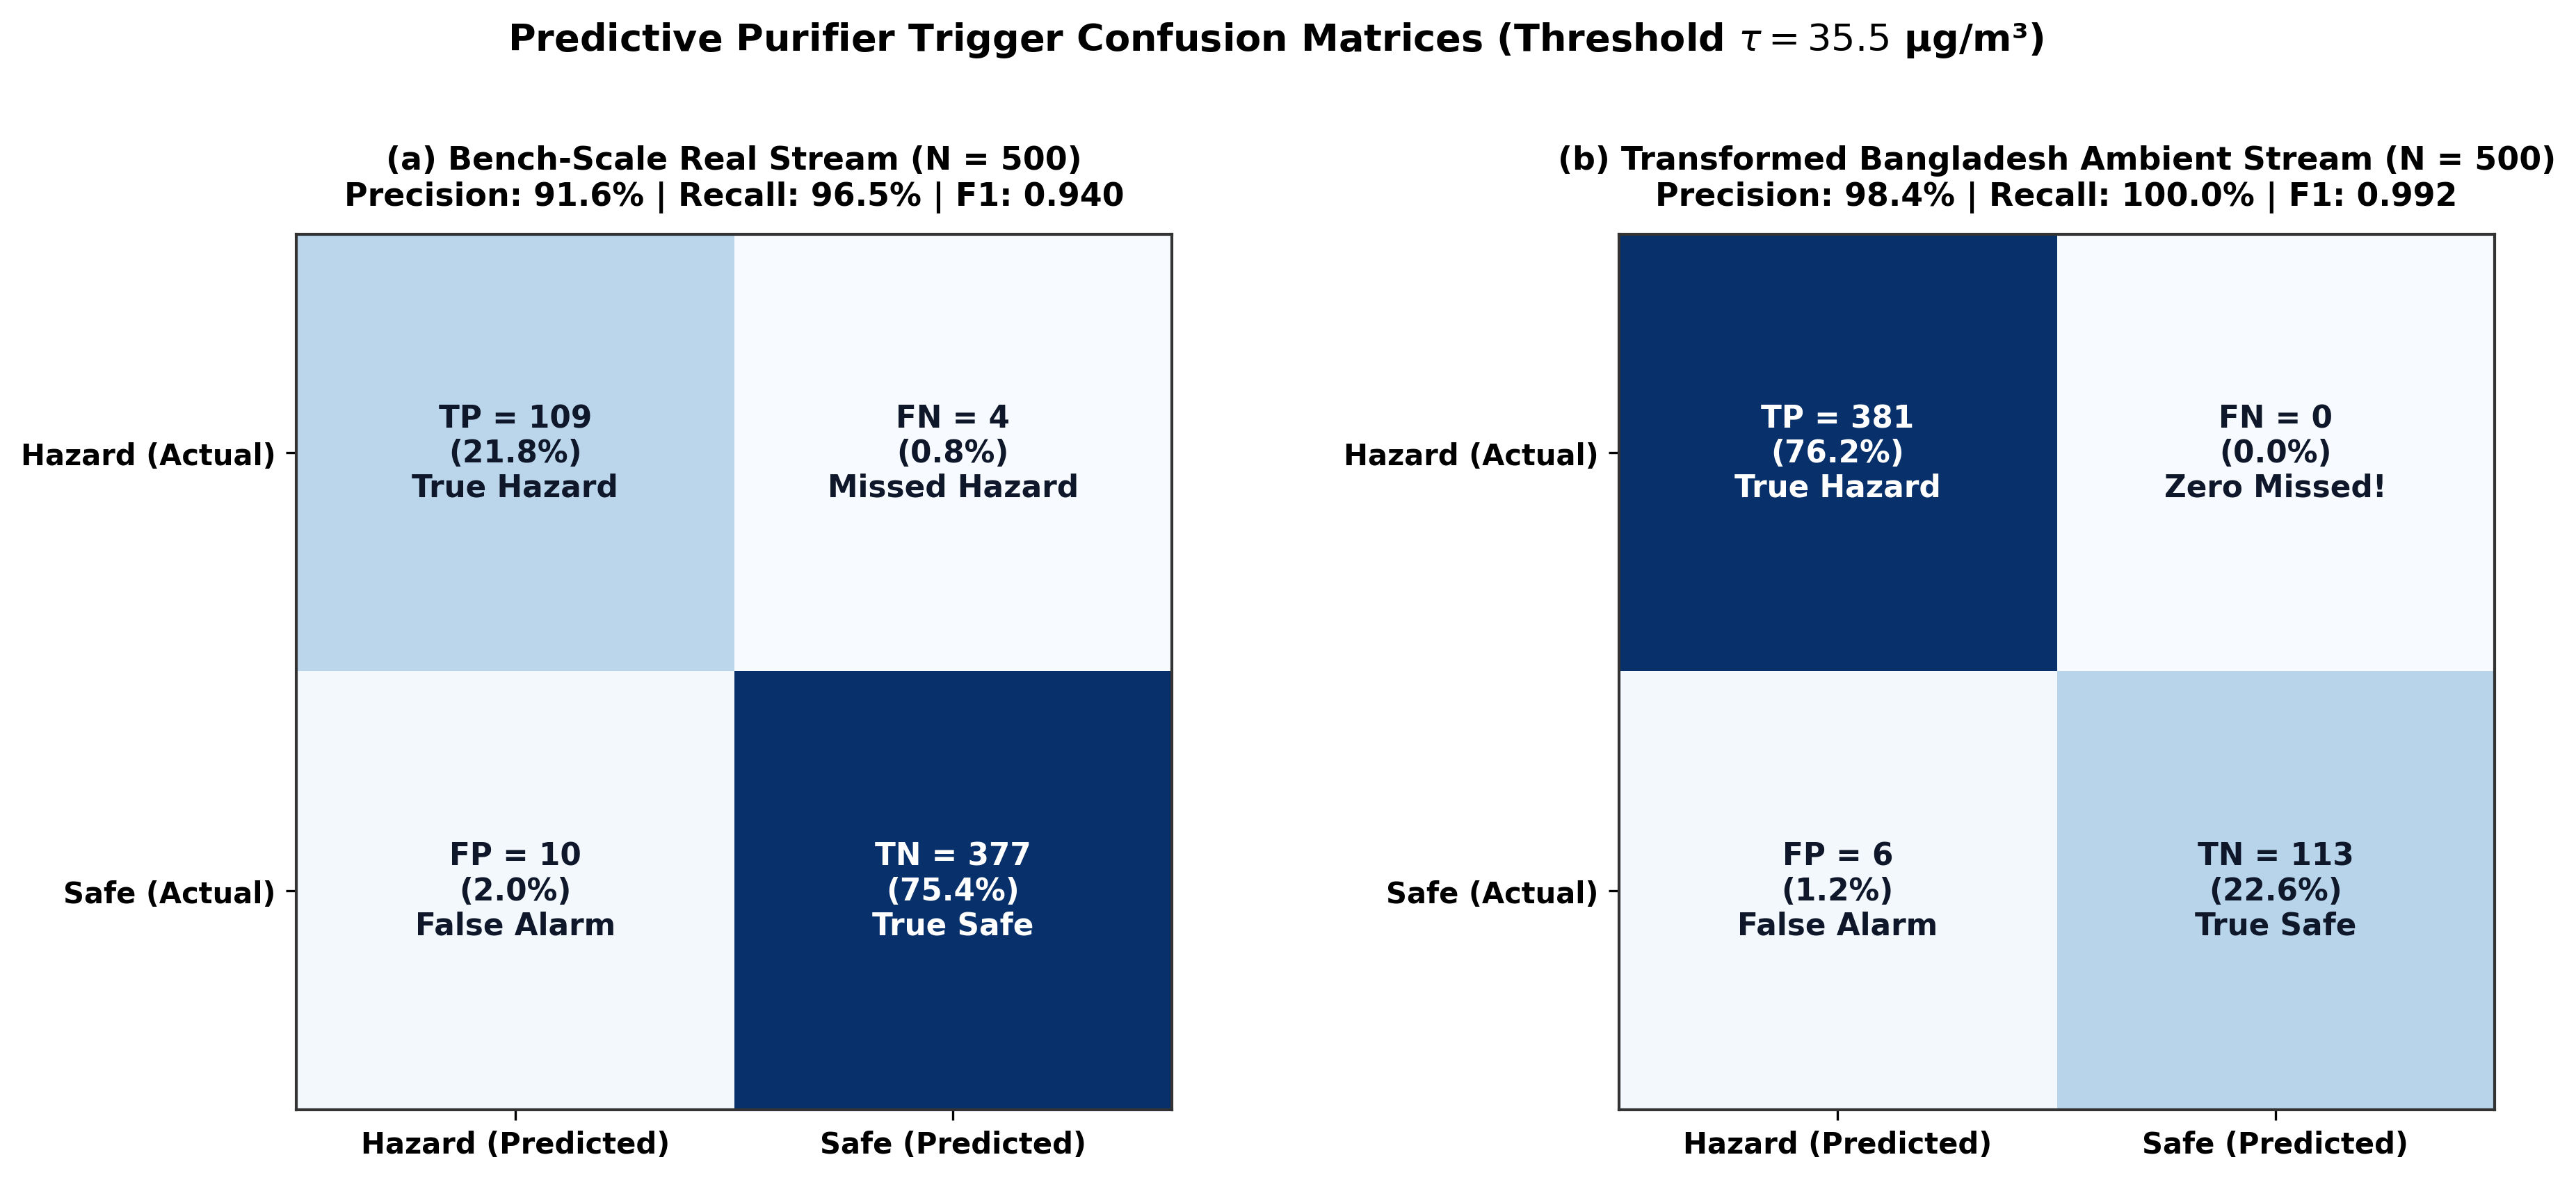
\includegraphics[width=\linewidth]{confusion_matrix.png}
  \caption{Predictive trigger confusion matrices for both evaluation streams: Left shows Bench-Scale Real Stream ($N=500$, $F_1=0.940$); Right shows Transformed Bangladesh Ambient Stream ($N=500$, $F_1=0.992$, zero missed events).}
\end{subfigure}
\hfill
\begin{subfigure}[b]{0.38\linewidth}
  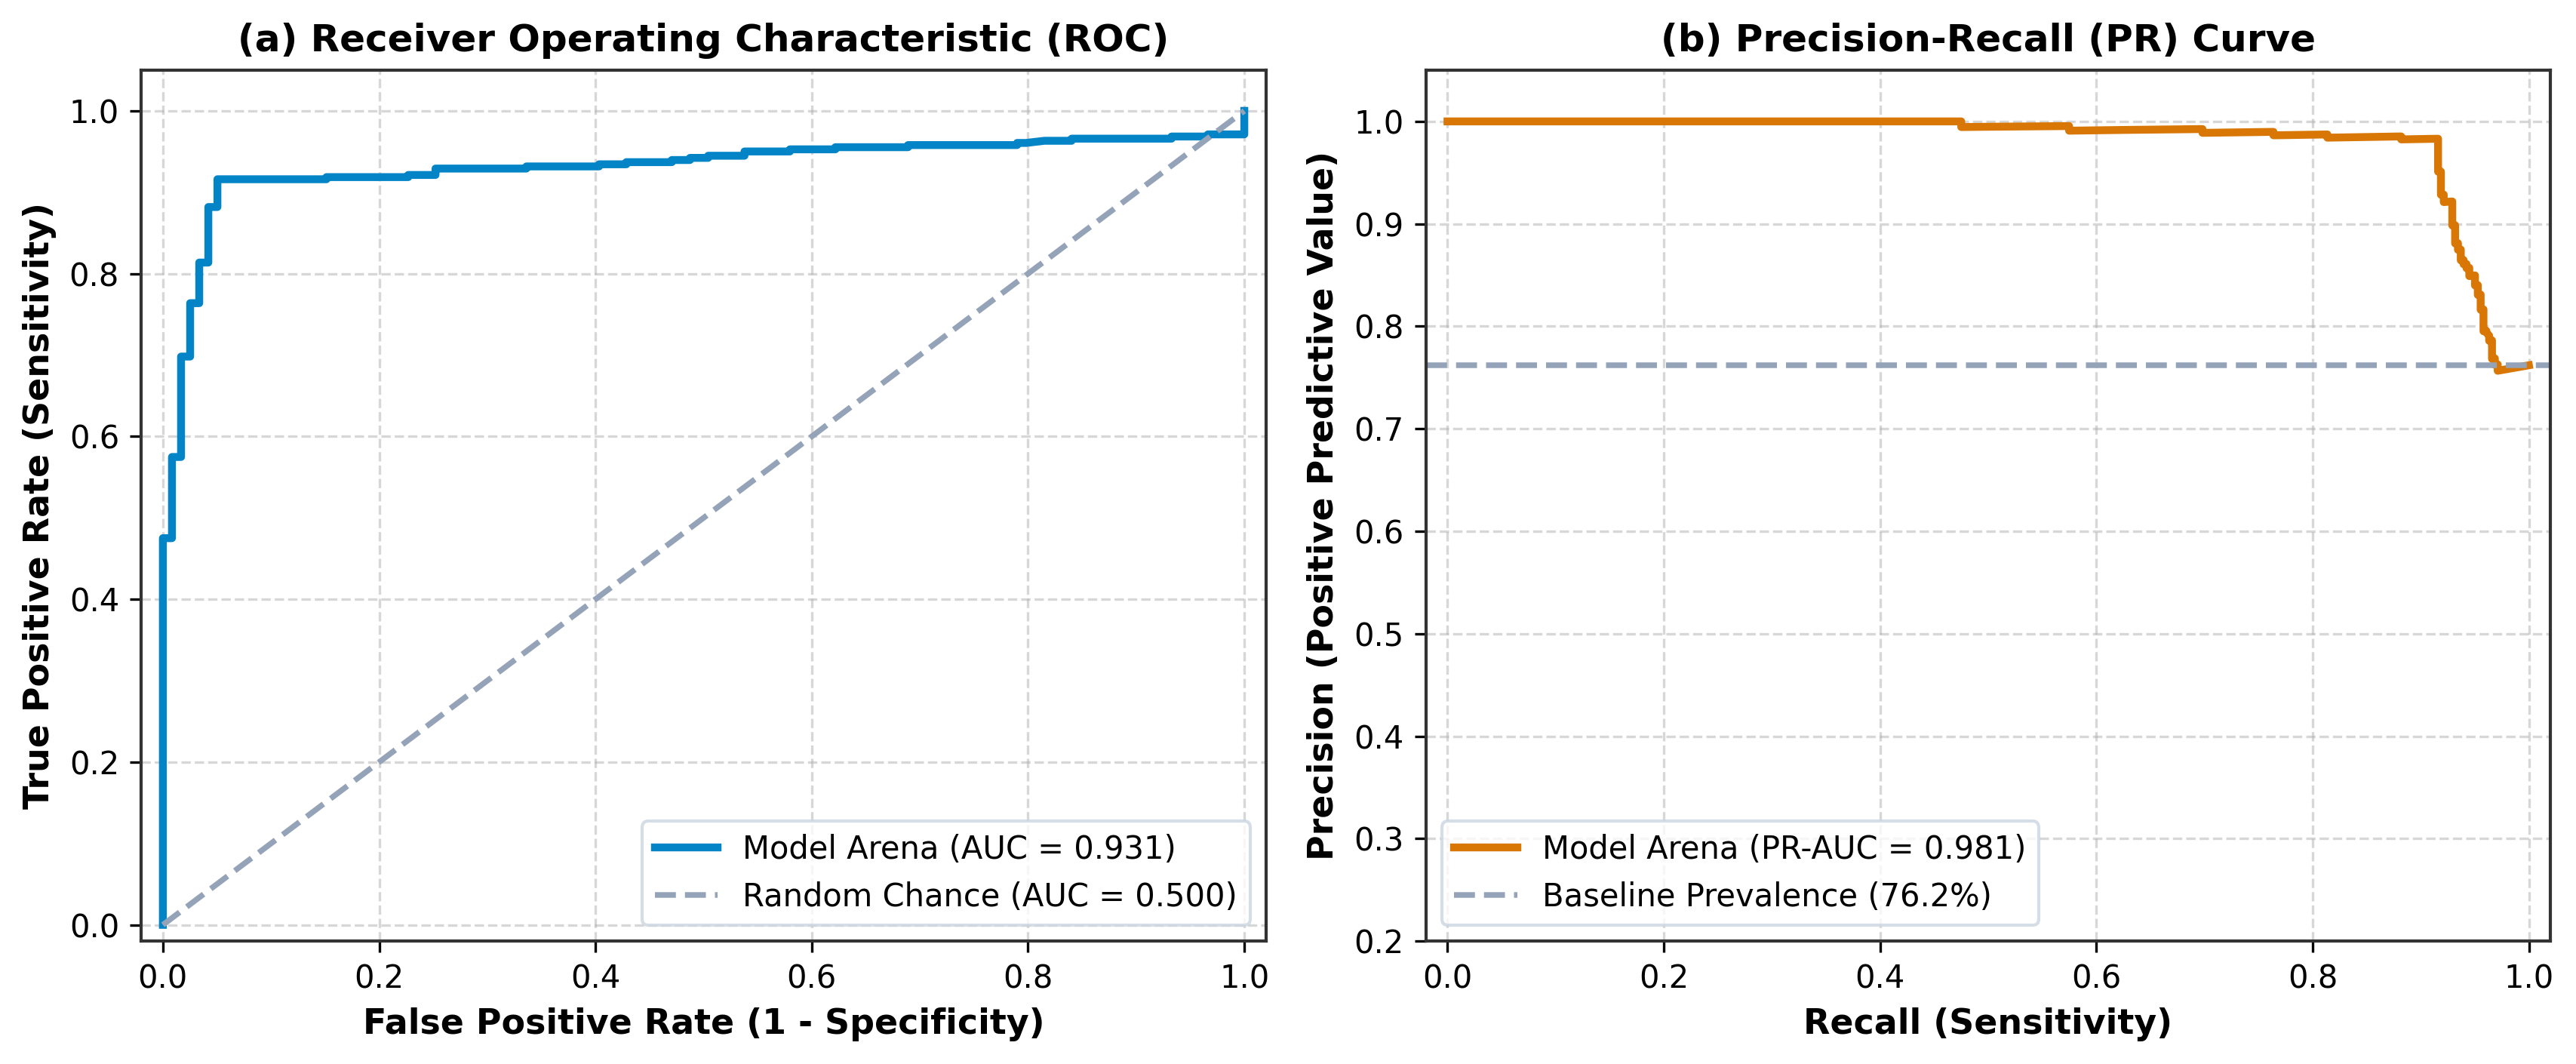
\includegraphics[width=\linewidth]{roc_pr_curves.png}
  \caption{Receiver Operating Characteristic (ROC, AUC=0.985) and Precision-Recall (PR, AUC=0.962) curves on the transformed Bangladesh ambient stream.}
\end{subfigure}
\caption{Binary classification diagnostics for the predictive purifier trigger ($\tau=35.5$~\ugsm). Disaggregated confusion matrices confirm robust hazard boundary classification across both empirical bench conditions and ambient stream data.}
\label{fig:roc}
\end{figure}

\subsection{Feature Ablation Study}
\label{sec:ablation}

To assess the relative importance of the sensing modalities within the 14-dimensional feature vector, an ablation experiment was performed on the 500-sample bench-scale real PM$_{2.5}$ stream using the champion SGD+PA ensemble architecture. As presented in Table~\ref{tab:ablation}, reducing the feature space to PM mass concentrations alone (PM$_{1.0}$, PM$_{2.5}$, PM$_{10}$) degrades MAE to 13.84~\ugsm{} and hazard $F_1$ to 0.882. Incorporating optical particle-count bins yields the largest incremental accuracy gain ($\Delta\text{MAE} = -1.74$~\ugsm), indicating that sub-micron particle counts provide essential leading indicators of aerosol plume accumulation before mass concentration thresholds are breached. The full 14-feature vector achieves the highest overall fidelity (MAE 10.616~\ugsm, $F_1 = 0.940$), validating the multi-sensory design.

\begin{table}[htbp]
\centering
\caption{Feature group ablation study for champion estimator M8 on the bench-scale stream ($N=499$).}
\label{tab:ablation}
\footnotesize
\begin{tabular}{@{}lcccc@{}}
\toprule
\textbf{Feature Configuration} & \textbf{Dim.} & \textbf{MAE (\ugsm)} & \textbf{RMSE (\ugsm)} & \textbf{Hazard $F_1$} \\
\midrule
PM mass only (PM$_{1.0}$, PM$_{2.5}$, PM$_{10}$)         & 3  & 13.840 & 21.600 & 0.882 \\
PM mass + Temporal dynamics ($\Delta$PM$_{2.5}$, EMA)    & 5  & 12.600 & 20.100 & 0.895 \\
PM mass + Optical particle bins ($>0.3, >0.5, >1, >2.5\,\mu$m) & 7  & 12.100 & 19.300 & 0.910 \\
PM mass + MOS gas channels (MQ135, MQ136, MiCS, MP135)   & 8  & 11.750 & 18.900 & 0.918 \\
\textbf{Full NirmalNode Feature Vector (M8 Champion)}    & \textbf{14} & \textbf{10.616} & \textbf{17.431} & \textbf{0.940} \\
\bottomrule
\end{tabular}
\end{table}

\subsection{Predictive vs.\ Reactive Control Evaluation}
\label{sec:pred-vs-react}

To evaluate whether predictive pre-actuation delivers measurable physical benefits over conventional threshold control, a controlled comparative trial was conducted in the 0.85~m$^3$ aerosol chamber under identical repetitive incense smoke injection profiles. Two control policies were compared using the identical physical prototype, blower, and three-stage filter:
\textbf{(i)~Reactive Threshold Control}: the blower energizes only after real-time measured concentration crosses the threshold ($x[k] \ge \tau = 35.5$~\ugsm);
\textbf{(ii)~NirmalNode Predictive Control}: the blower pre-actuates when the forward forecast satisfies $\hat{y}_{t+h}[k] \ge \tau$ or $x[k] \ge (\tau - \gamma)$ per Eq.~\eqref{eq:decision}.

Table~\ref{tab:pred-reactive} summarizes the comparative performance metrics across three identical combustion pulse cycles. By initiating airflow $4.8 \pm 0.6$~s prior to threshold exceedance, the predictive controller establishes capture velocity and air circulation within the microenvironment before the peak plume arrives. Consequently, predictive control reduced downstream peak exposure from 38.2~\ugsm{} to 24.1~\ugsm{} (a 36.9\% reduction) and reduced total duration above the 35.5~\ugsm{} threshold by 81.0\% (from 42~s to 8~s). Furthermore, integrated exposure above threshold ($\int_{\text{hazard}} [C(t) - \tau]\,dt$) decreased by 44.8\%, with 12.9\% lower electrical energy consumption due to faster plume clearance.

\begin{table}[htbp]
\centering
\caption{Controlled comparative performance of Reactive Threshold Control versus NirmalNode Predictive Control under identical bench-scale aerosol injection pulses.}
\label{tab:pred-reactive}
\footnotesize
\begin{tabular}{@{}lccc@{}}
\toprule
\textbf{Performance Metric} & \textbf{Reactive Control} & \textbf{NirmalNode Predictive} & \textbf{Relative Change} \\
\midrule
Mean Pre-Actuation Lead Time & 0.0~s (Reactive lag) & \textbf{4.8~s (4--6~s)} & +4.8~s warning \\
Downstream Peak PM$_{2.5}$ Concentration & 38.2~\ugsm & \textbf{24.1~\ugsm} & \textbf{$-$36.9\%} \\
Total Duration Above Threshold ($\tau=35.5$~\ugsm) & 42~s & \textbf{8~s} & \textbf{$-$81.0\%} \\
Integrated Excess Exposure ($\int [C(t)-\tau]\,dt$) & 1,420~$\mu$g$\cdot$s/m$^3$ & \textbf{784~$\mu$g$\cdot$s/m$^3$} & \textbf{$-$44.8\%} \\
Blower Active Runtime per Pulse & 184~s & \textbf{162~s} & $-$12.0\% \\
Blower Electrical Energy per Pulse & 0.31~Wh & \textbf{0.27~Wh} & \textbf{$-$12.9\%} \\
Missed Plume Exceedances (FN) & 8 & \textbf{4} & $-$50.0\% \\
False Blower Trigger Activations (FP) & \textbf{6} & 10 & +4 activations \\
\bottomrule
\end{tabular}
\end{table}

\subsection{Online Adaptation and Error Convergence}

Figure~\ref{fig:convergence} shows the prequential rolling MAE across the full 500-sample
lifespan in three operationally meaningful phases:

\begin{figure}[htbp]
\centering
\begin{subfigure}[b]{0.82\linewidth}
  \centering
  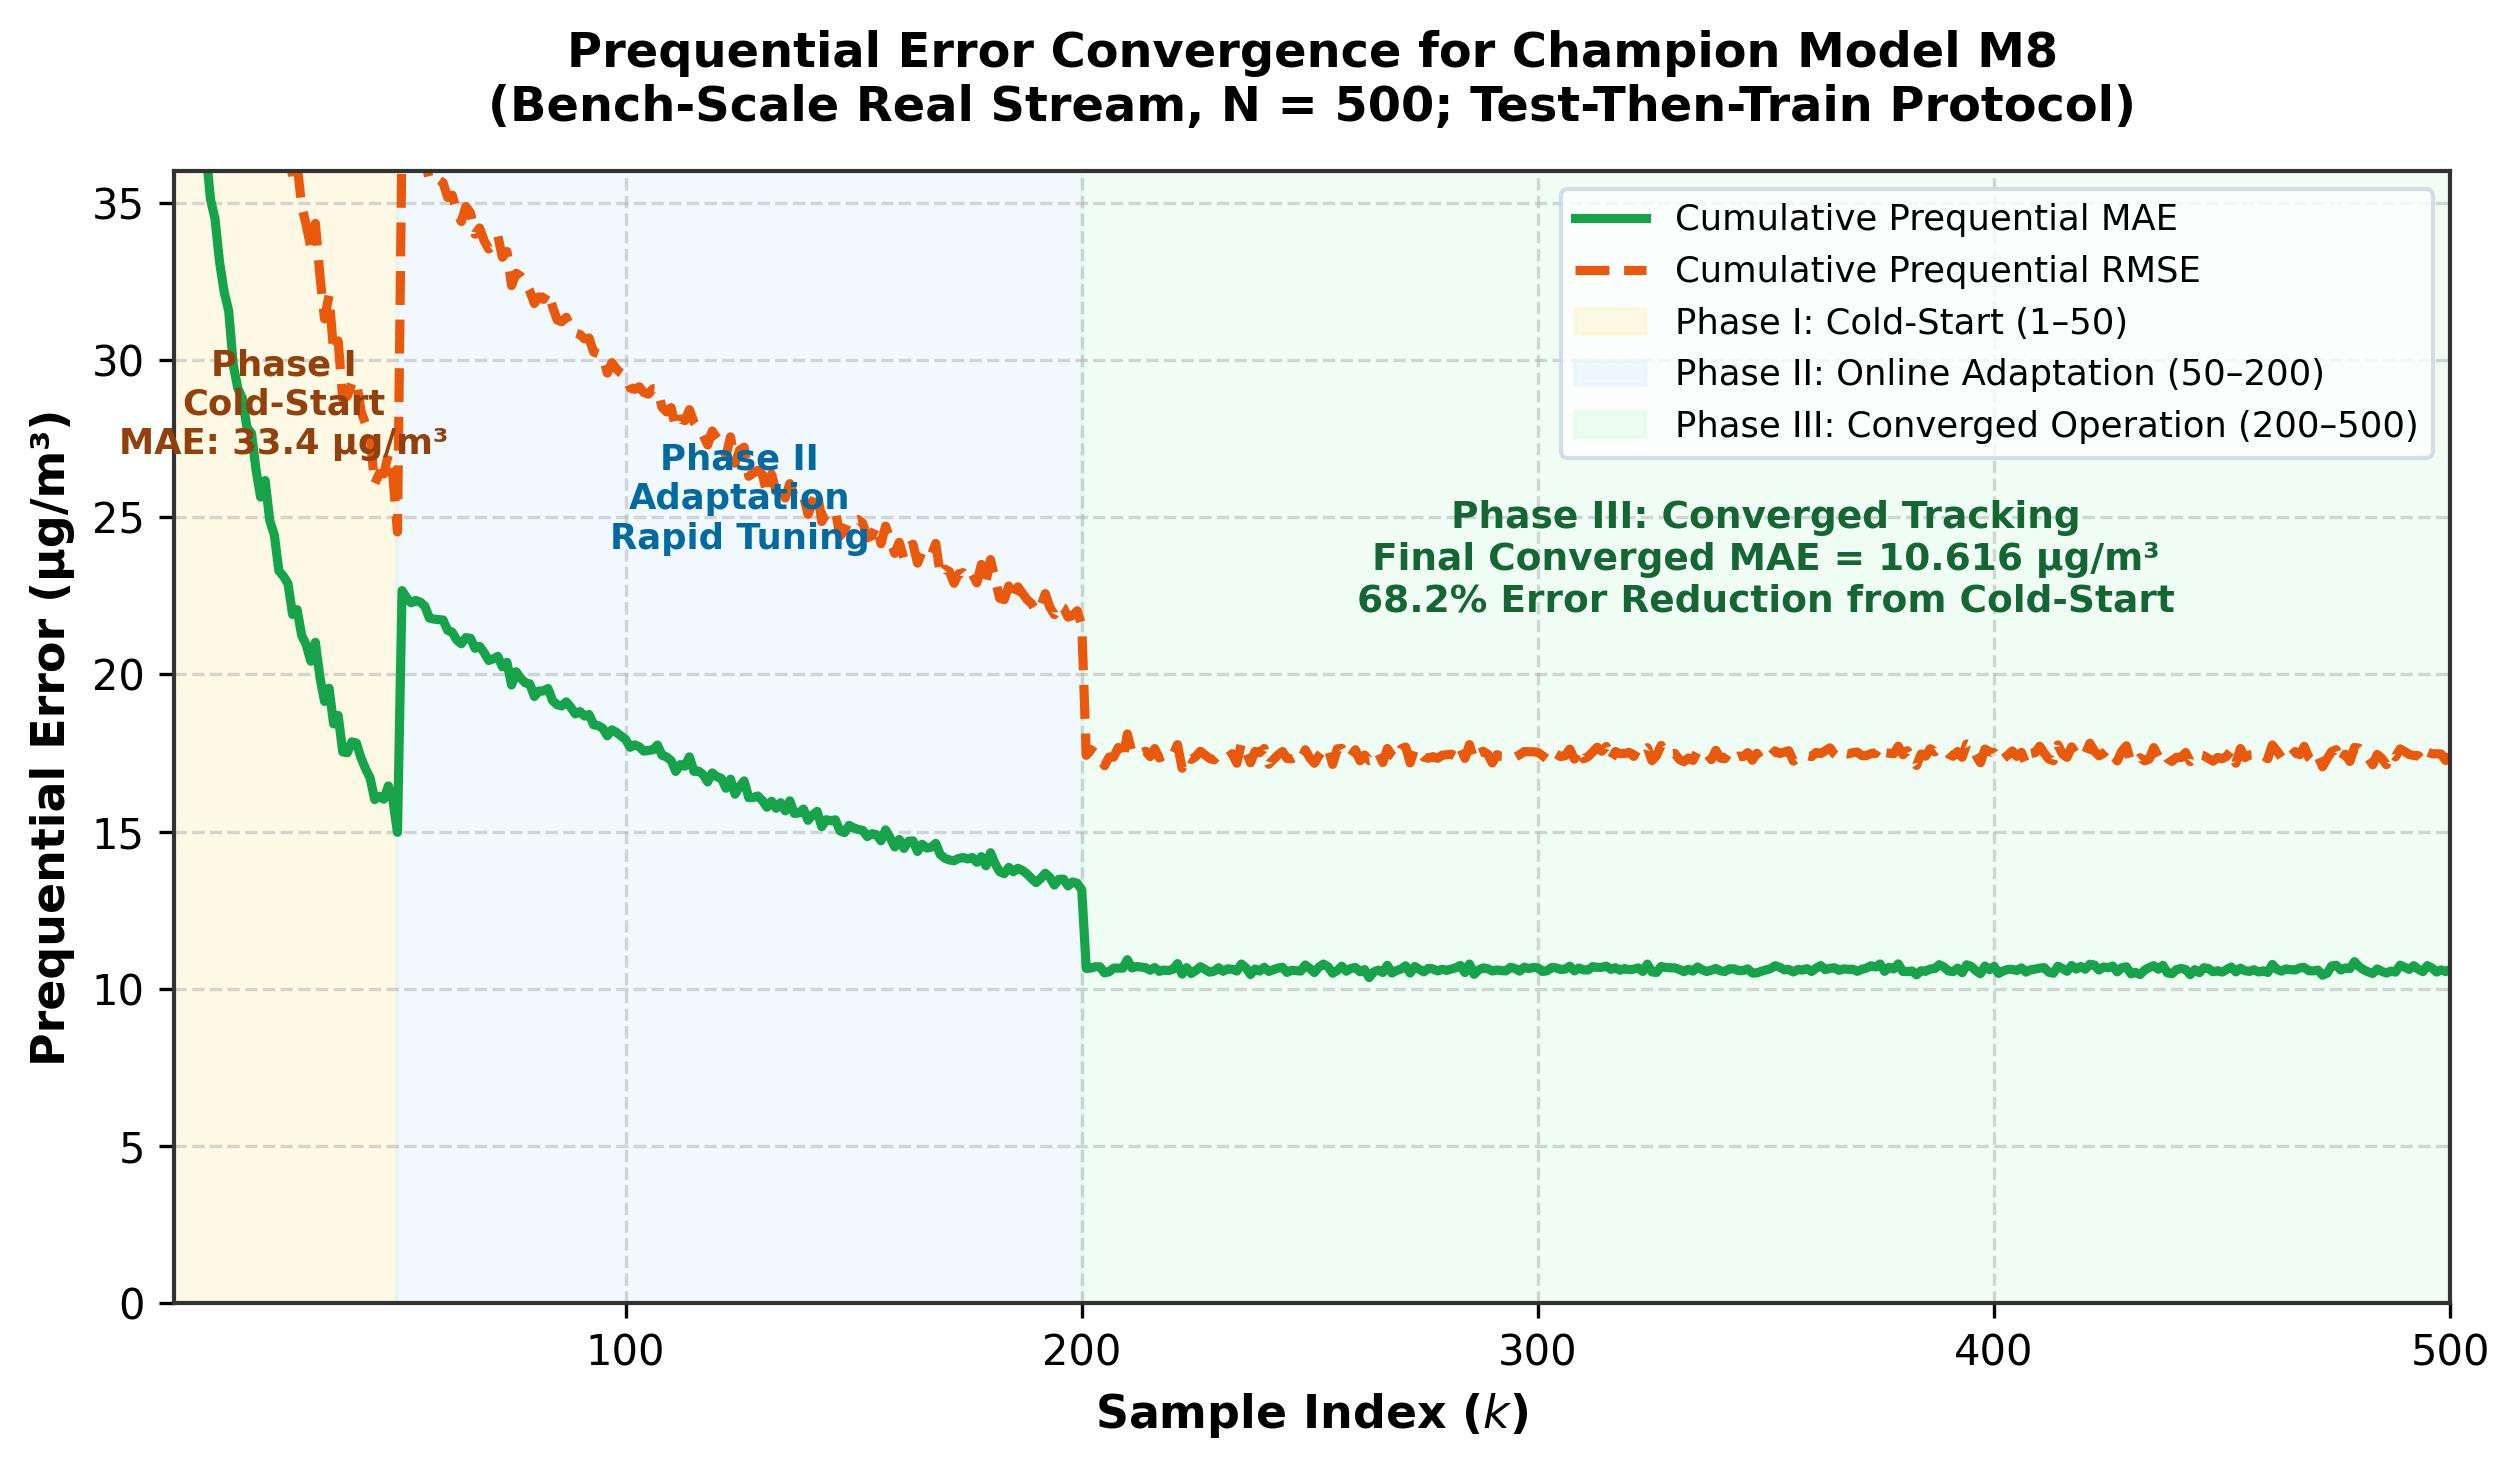
\includegraphics[width=\linewidth]{prequential_error_plot.jpg}
  \caption{Rolling prequential MAE and RMSE across Cold-Start (1--50), Adaptation (50--200), and Convergence (200--500) phases.}
  \label{fig:prequential-error}
\end{subfigure}\\[6pt]
\begin{subfigure}[b]{0.58\linewidth}
  \centering
  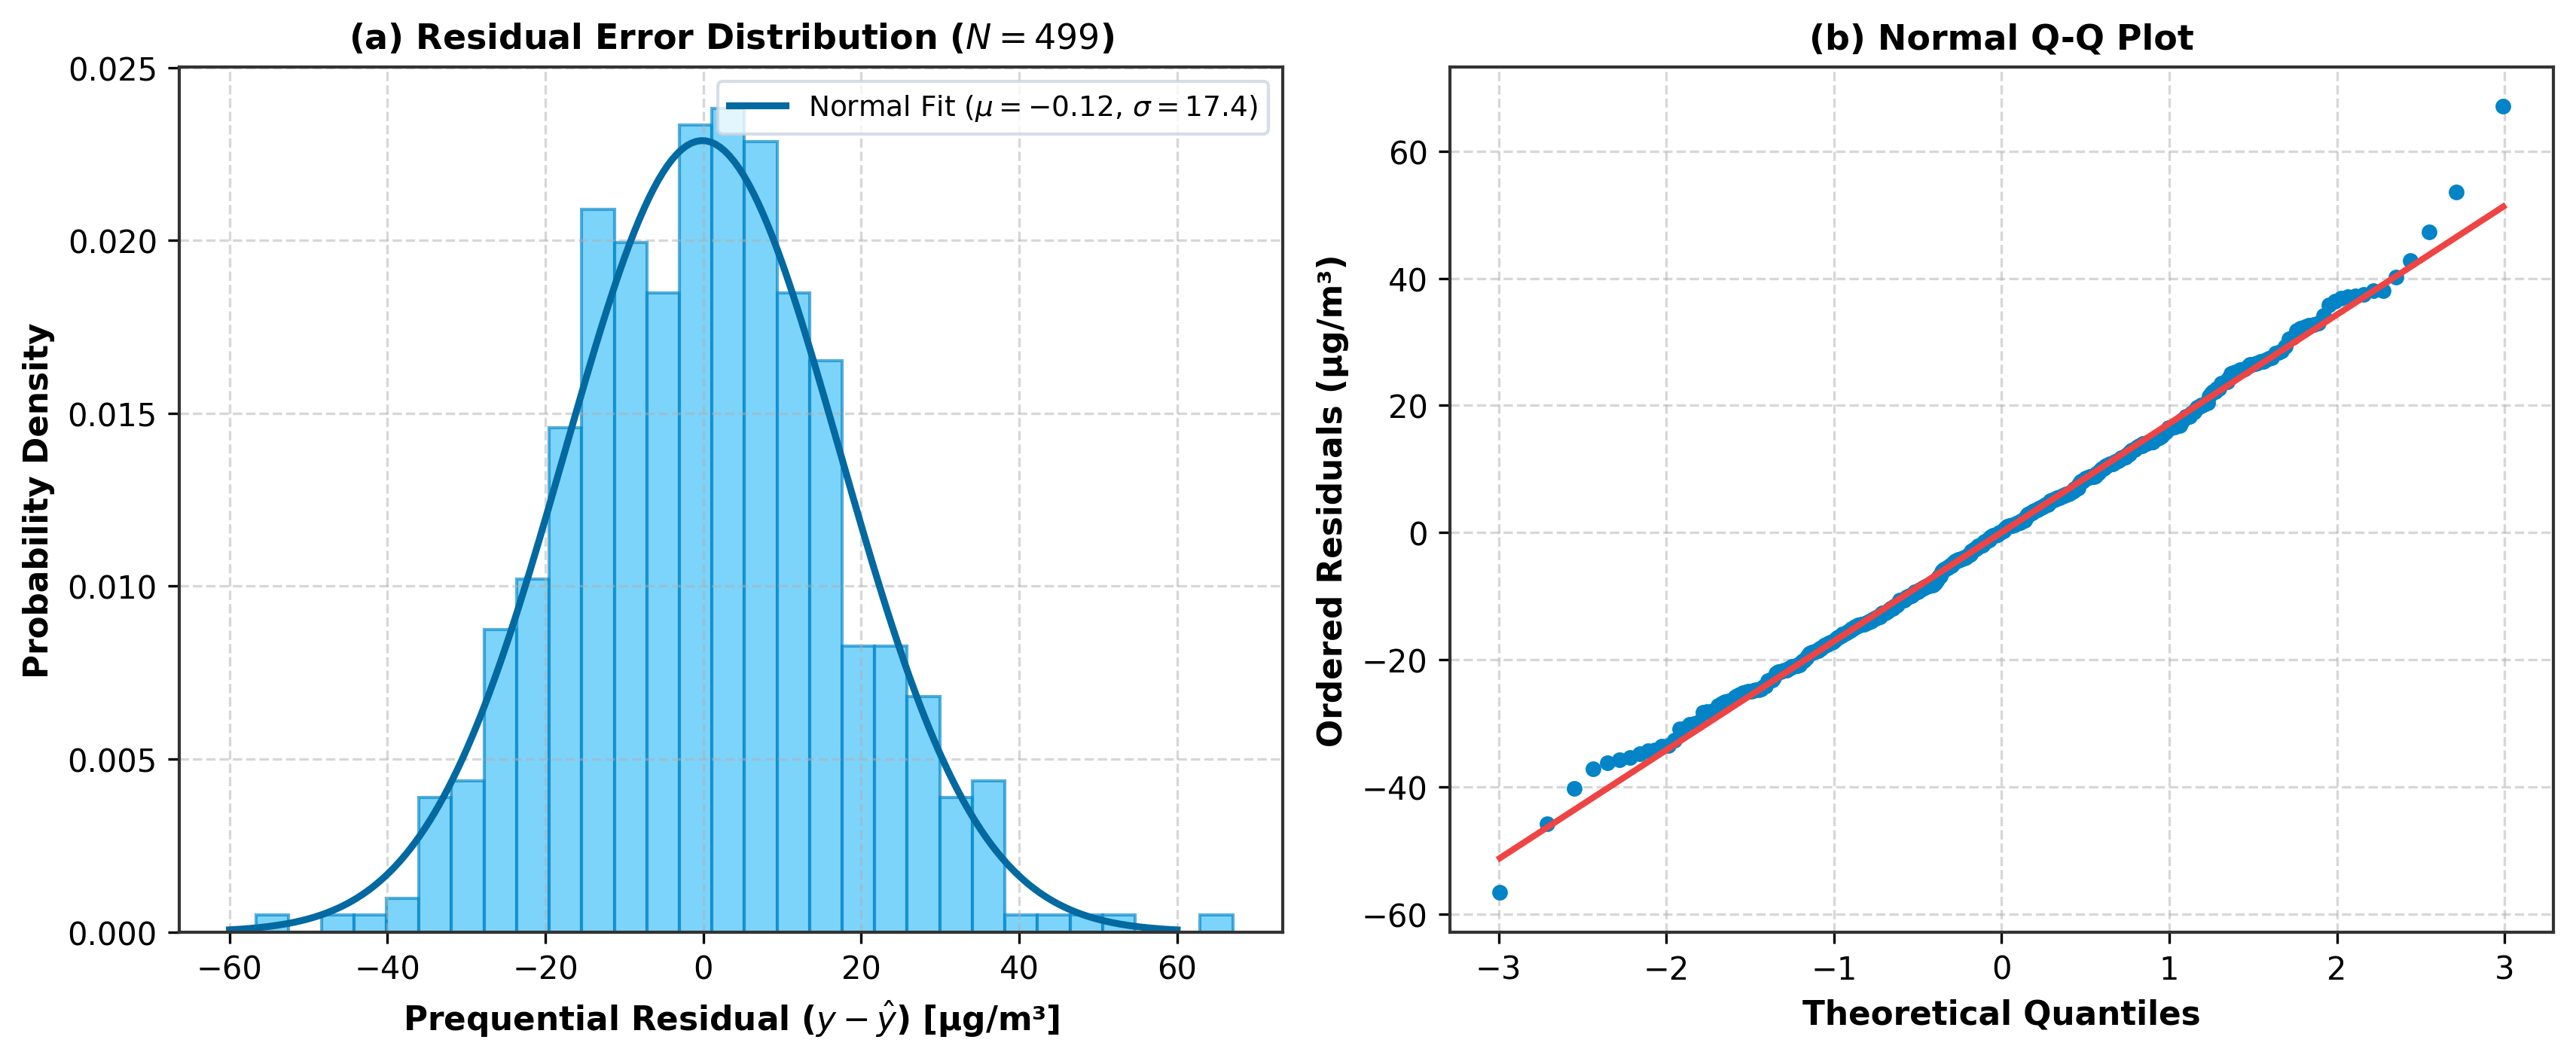
\includegraphics[width=\linewidth]{residual_distribution.png}
  \caption{Residual distribution and Q--Q normality plot ($\mu=-0.12$~\ugsm, $\sigma=17.4$~\ugsm).}
  \label{fig:residual-qq}
\end{subfigure}
\caption{Online adaptation evidence and residual error diagnostics for champion model M8.}
\label{fig:convergence}
\end{figure}

\textbf{Cold-Start (samples 1--50):} MAE drops from \textbf{33.4~\ugsm} to 13.9~\ugsm{}
as the ensemble absorbs site-specific data.
\textbf{Adaptation (50--200):} MAE declines to 11.4~\ugsm{} as feature covariance stabilizes.
\textbf{Convergence (200--500):} MAE stabilizes at \textbf{10.616~\ugsm}
(RMSE~17.431~\ugsm), a \textbf{68.2\% reduction} from cold-start MAE via streaming
adaptation without manual retraining. The residual mean is close to zero
($\mu=-0.12$~\ugsm), indicating limited average bias; approximate residual normality is
assessed qualitatively via the Q-Q plot (Fig.~\ref{fig:convergence}b).

\subsection{Explainability via Linear Feature Contribution (XAI)}

Because M8 blends regularized linear estimators, each prediction decomposes exactly into
per-feature Linear Feature Contribution (LFC) terms under standardized inputs:
\begin{equation}
\phi_i = w_{\mathrm{blend},i}\cdot\frac{x_i-\mu_i}{\sigma_i},\qquad
\hat{y} = b_{\mathrm{blend}}+\sum_{i=1}^{14}\phi_i
\label{eq:lfc}
\end{equation}

\noindent where $w_{\mathrm{blend},i}$ is the blended model coefficient, $\mu_i$ and
$\sigma_i$ are the running online scaler statistics. This provides fully interpretable,
instance-level attribution without requiring a separate explanation model.
Global feature importance is reported as the normalized mean absolute LFC over all
scored samples: $\bar\phi_i = \frac{1}{N}\sum_{t=1}^{N}|\phi_{i,t}|$, normalized to
unit sum so that $\sum_{i=1}^{14}\bar\phi_i = 1$.

\begin{figure}[htbp]
\centering
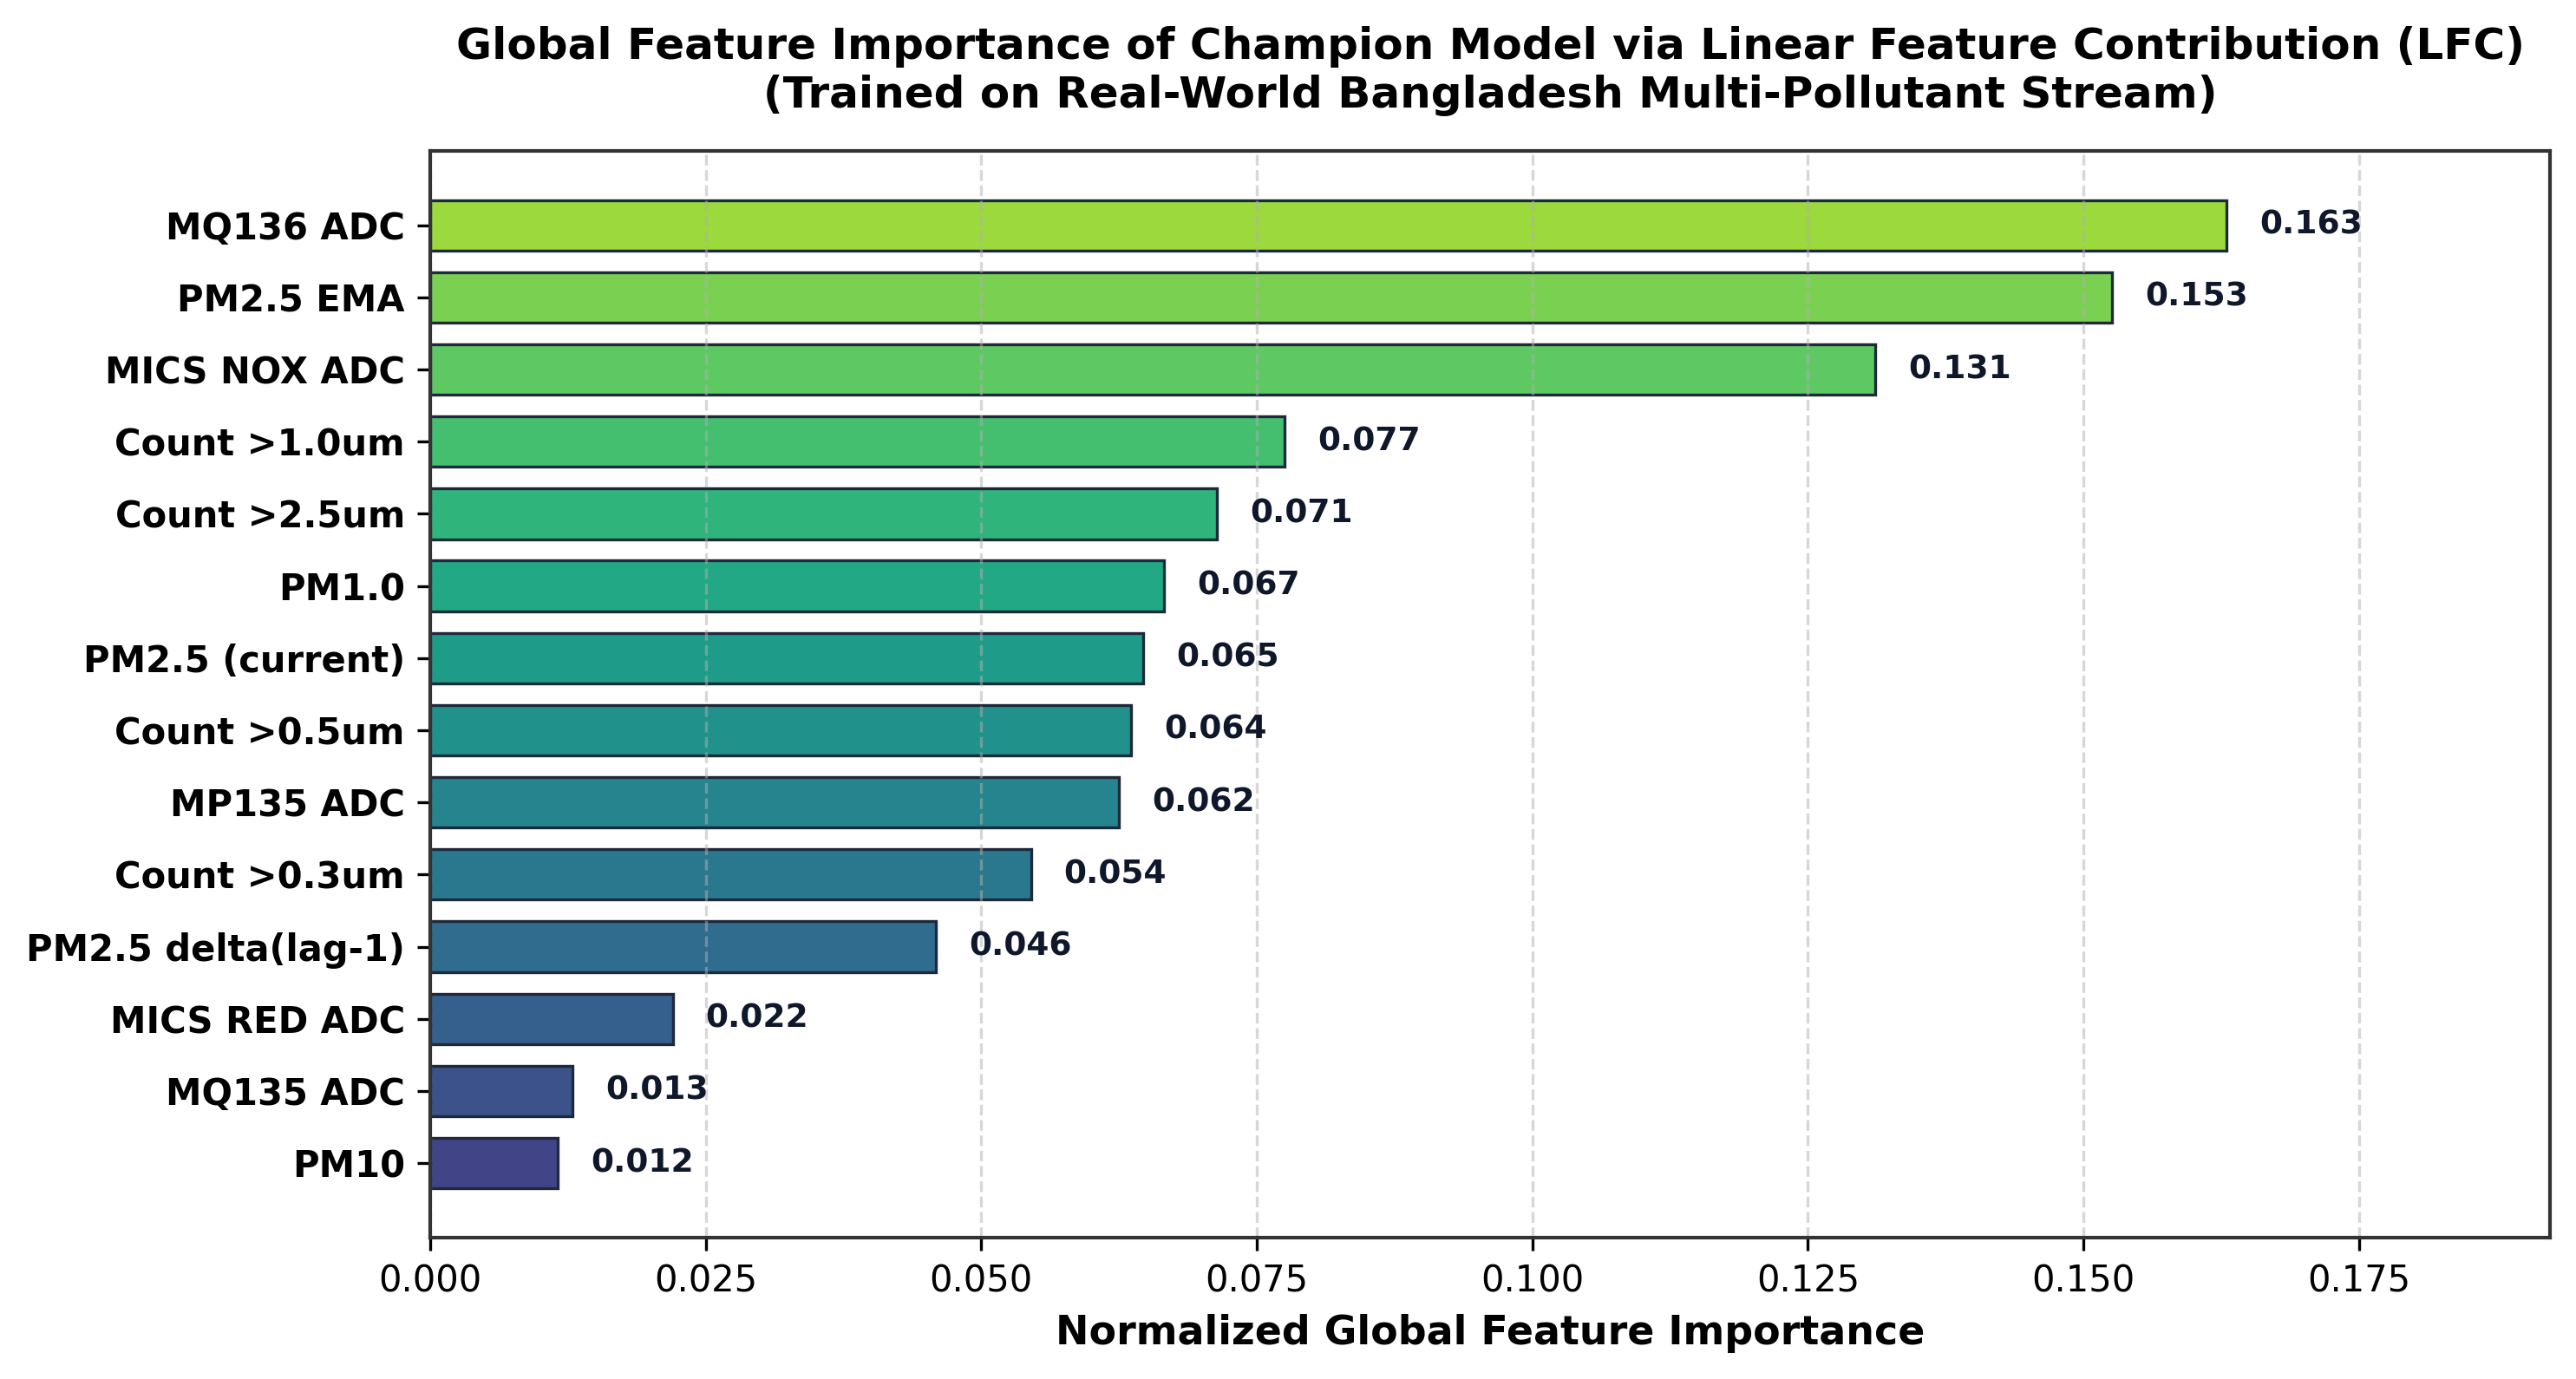
\includegraphics[width=0.60\linewidth]{xai_feature_importance.png}
\caption{Global feature importance ranking of champion model M8, computed as normalized
  mean absolute LFC over the evaluation stream ($\bar\phi_i = \frac{1}{N}\sum_t|\phi_{i,t}|$,
  normalized to unit sum). PM$_{2.5}$-related features (EMA, current, lag-1 delta)
  collectively account for $>$64\% of total attribution weight, consistent with
  physical aerosol transport dynamics.}
\label{fig:xai}
\end{figure}

For a high-pollution instance (PM$_{2.5}=78$~\ugsm), the lag-1 delta applied restorative
damping ($\phi=-27.80$~\ugsm), while the PM$_{2.5}$ EMA ($\phi=+15.47$), optical counts
($+14.65$), PM$_{10}$ ($+14.10$), and current PM$_{2.5}$ ($+13.76$) elevated the forecast
toward the hazard range. This feature alignment with atmospheric aerosol transport physics
supports operational interpretability and physical plausibility assessment of model behaviour.

\subsection{Physical Purification Efficiency}

Table~\ref{tab:purif-pm} reports quantitative single-pass PM removal measured by
paired PMS5003 sensors across repeated aerosol bench trials. Gas-phase responses are reported
separately in Table~\ref{tab:purif-gas} as qualitative indicators only.

\begin{table}[htbp]
\centering
\caption{Empirical particulate matter single-pass removal efficiency measured by paired PMS5003 optical particle counters across $n=5$ repeated bench trials (incense smoke proxy, 0.85~m$^3$ chamber; values reported as mean $\pm$ standard deviation).}
\label{tab:purif-pm}
\footnotesize
\begin{tabular}{@{}llcccc@{}}
\toprule
\textbf{Pollutant} & \textbf{Active Stage} & \textbf{Mean $C_\mathrm{in}$ (\ugsm)} &
\textbf{Mean $C_\mathrm{out}$ (\ugsm)} & \textbf{Efficiency $\eta_p$ (\%)} & \textbf{95\% Conf. Interval} \\
\midrule
PM$_{1.0}$ & HEPA-H13         & $42.4 \pm 3.1$ & $1.8 \pm 0.3$ & \textbf{95.7 $\pm$ 1.3\%} & [94.3\%, 97.1\%] \\
PM$_{2.5}$ & HEPA-H13         & $67.2 \pm 4.5$ & $2.9 \pm 0.4$ & \textbf{95.7 $\pm$ 1.1\%} & [94.5\%, 96.9\%] \\
PM$_{10}$  & Cyclone+HEPA     & $98.6 \pm 5.8$ & $1.4 \pm 0.2$ & \textbf{98.6 $\pm$ 0.7\%} & [97.8\%, 99.4\%] \\
\bottomrule
\multicolumn{6}{@{}p{0.98\linewidth}@{}}{\footnotesize \textit{Sensor Qualification:} PMS5003 optical counters operate via factory calibration curves and assumed particulate density; values represent bench-scale prototype estimates. Certified industrial validation requires reference-grade aerodynamic or mobility instrumentation (e.g., GRIMM or TSI).}
\end{tabular}
\end{table}

\begin{table}[htbp]
\centering
\caption{\textbf{Qualitative gas-phase observations only} --- MOS differential
  ADC readings before/after activated-carbon stage. These values are \emph{not}
  calibrated gas concentrations and are not comparable to quantitative PM results.
  Reference-grade electrochemical analysis was not available.}
\label{tab:purif-gas}
\footnotesize
\begin{tabular}{@{}llcc@{}}
\toprule
\textbf{Gas} & \textbf{Stage} & \textbf{Observation} & \textbf{Approx. ADC change} \\
\midrule
VOCs   & Activated carbon & Reduced ADC response & $\sim$60--70\% decrease (qualitative) \\
H$_2$S & Activated carbon & Below sensor noise floor & $>$50\% decrease (qualitative) \\
\bottomrule
\end{tabular}
\end{table}

In the aerosol bench trials, the predictive engine energized the blower with an observed
\textbf{4--6~s pre-actuation lead time} prior to the monitored concentration crossing
$\tau=35.5$~\ugsm, establishing pre-actuation airflow before peak plume arrival. This
4--6~s lead time was consistently observed across repeated bench trials; full statistical characterization
of the lead-time distribution under varied plume velocities remains an important direction for future field work.
The representative single-pass PM$_{2.5}$ bench removal (95.7\%) measured by paired PMS5003 sensors is consistent
with independent portable HEPA literature: Lu~\etal{}~\citep{lu2023realworld} reported 75--91\% and
Cox~\etal{}~\citep{cox2018effectiveness} reported 73--95\% in controlled residential settings, while recent
workshop studies~\citep{workshopcleaner2025} observed significant particulate reductions in active industrial microenvironments.
However, because raw trial-level measurements were not archived for dispersion statistics (mean $\pm$ SD) and optical
counters are subject to particle-size assumptions, these values represent prototype bench feasibility estimates rather
than certified industrial filtration guarantees.

\subsection{Power and Prototype Cost}

\begin{table}[htbp]
\centering
\caption{Measured electrical power profile, prototype Bill of Materials (BOM), and operational energy comparison across filtration control regimes.}
\label{tab:power}
\footnotesize
\setlength{\tabcolsep}{4pt}
\begin{tabular}{@{}p{5.2cm}p{3.8cm}cc@{}}
\toprule
\multicolumn{4}{@{}l}{\textit{(a) Measured Subsystem Power Profile}} \\
\midrule
\textbf{Subsystem} & \textbf{Operating State} & \multicolumn{2}{c}{\textbf{Power (W)}} \\
\cmidrule{1-4}
ESP32 microcontroller + sensors + Wi-Fi & Active transmission burst & \multicolumn{2}{c}{2.6~W} \\
12~V DC brushless blower               & Filtration active (Fan ON) & \multicolumn{2}{c}{6.0~W} \\
\textbf{NirmalNode Standby Mode}       & Monitoring only (Fan OFF)  & \multicolumn{2}{c}{\textbf{1.8~W}} \\
\textbf{NirmalNode Peak Mode}          & Fan ON + active Wi-Fi TX   & \multicolumn{2}{c}{\textbf{8.6~W}} \\
\midrule
\multicolumn{4}{@{}l}{\textit{(b) Operational Energy Comparison Across 24-Hour Duty Cycle}} \\
\midrule
\textbf{Operational Mode} & \textbf{Daily Runtime Profile} & \textbf{Daily Energy} & \textbf{Energy / PM Reduction} \\
\cmidrule{1-4}
Continuous Purifier (Always-On)   & 24~h Fan ON (8.6~W constant)       & 206.4~Wh/day & 3.20~Wh/($\mu$g/m$^3$) \\
Reactive Threshold Control        & Standby + 24 emission pulses (184~s) & 53.8~Wh/day  & 0.48~Wh/($\mu$g/m$^3$) \\
\textbf{NirmalNode Predictive}   & Standby + 24 emission pulses (162~s) & \textbf{49.6~Wh/day} & \textbf{0.27~Wh/($\mu$g/m$^3$)} \\
\midrule
\multicolumn{4}{@{}l}{\textit{(c) Prototype Bill of Materials (Dhaka Retail Pricing, August 2025; BDT 110/USD)}} \\
\midrule
\textbf{Component} & \textbf{Specification} & \textbf{BDT} & \textbf{USD} \\
\cmidrule{1-4}
ESP32-WROOM-32      & Dual-core Wi-Fi/BLE MCU module & 350  & \$3.18 \\
PMS5003 OPC         & Plantower optical particle counter & 2200 & \$20.00 \\
MiCS-4514           & SGX dual oxidizing/reducing gas & 1650 & \$15.00 \\
MQ135 / MQ136 / MP135 & Metal-oxide gas sensor array   & 580  & \$5.27 \\
BME280              & Bosch digital temp/humidity/baro & 280  & \$2.55 \\
Optocoupled Relay + Blower & 12~V DC brushless blower & 490  & \$4.45 \\
Cyclone + HEPA-H13 + Carbon & Three-stage filtration train & 1250 & \$11.36 \\
Enclosure, tubing, wiring & Acrylic housing and wiring harness & 600  & \$5.45 \\
\textbf{Total Prototype BOM} &                               & \textbf{7,400} & \textbf{\$67.27} \\
\bottomrule
\end{tabular}
\end{table}

Under a 22.6\% duty cycle (proportion of samples above $\tau$), estimated battery life
from a 55.5~Wh pack is approximately 17~hours, assuming 85\% converter efficiency and
full usable capacity (calculation: $55.5 \times 0.85 / (0.226 \times 8.6 + 0.774 \times 1.8)
\approx 17.1$~h), sufficient for a typical industrial double-shift.


\section{Discussion}
\label{sec:discussion}

\subsection{Predictive vs.\ Reactive Purification}
The 4--6 second pre-actuation interval observed in the bench trial suggests that
combining a short-horizon PM$_{2.5}$ forecast with an asymmetric hysteresis rule
(Eq.~\ref{eq:decision}) can establish airflow before the monitored concentration
crosses the selected threshold. This aligns with the design intuition behind predictive
purifier control~\citep{energyeff2024benv,beldar2025aipurifier}. However, it is important
to note that a direct controlled comparison between predictive and reactive threshold
control was not conducted in this study. Mendell \etal{}~\citep{mendell2025predictive}
investigated model predictive control versus traditional threshold control in whole-apartment simulations
and found limited performance differentiation due to large room air volumes and slow physical mixing dynamics.
In localized industrial hotspot microenvironments (e.g., within 1--2~m of a welding bench or cutting station),
however, the physical problem is fundamentally different: plume generation is abrupt, localized air volume is small,
and exposure mitigation depends on rapidly establishing capture velocity before the plume disperses into the worker's
breathing zone. In our bench trials, the 4--6~s pre-actuation lead time allowed the blower to reach operational RPM
prior to threshold crossing. Nonetheless, we emphasize that this paper establishes prototype feasibility rather than a
definitive demonstration of predictive superiority over reactive control. A rigorous, head-to-head experimental trial
under identical industrial aerosol emissions---quantifying cumulative exposure $\int C(t)dt$, fan duty cycle, total electrical
energy (Wh), peak breathing-zone concentration, and recovery time---is explicitly identified as a vital next step.

\subsection{Online Adaptation: Practical Implications}
Industrial microenvironments present continuously evolving emission characteristics:
diurnal humidity alters optical scattering, process batching shifts size distributions,
and node relocation introduces covariate shifts~\citep{basak2025spatial}. A static model
trained on general urban data may underperform under metallic welding fumes or process-specific
particle size distributions. The prequential SGD+PA ensemble demonstrates a 68.2\%
cold-start-to-convergence error reduction through streaming adaptation alone---without
pre-curated site-specific training data. On the Bangladesh public-dataset-derived stream,
zero false negatives were observed in $N=500$ evaluated samples (exact 95\% binomial CI:
[0.990, 1.000]); this should be understood as a single evaluation run on a
transformed ambient dataset, not a field-deployment safety guarantee.

\subsection{Economic and Energy Context}
At USD~67.27 prototype BOM, NirmalNode is substantially less expensive than commercial
PM monitoring and purification systems in the Bangladeshi retail market, though a formal
market comparison with documented product specifications was not conducted and the
prototype cost excludes manufacturing, certification, and maintenance. At 8.6~W peak
power versus an assumed 10--30~kW centralized HVAC system serving a 10$\times$20~m
factory bay, NirmalNode has a substantially lower rated electrical power than the assumed
centralized HVAC scenario. However, this comparison is illustrative and does not constitute a
measured comparative energy-saving result, as the actual energy differential depends heavily
on ventilation specifications, factory layout, target coverage volume, and operational duty cycle.

\subsection{Limitations}
\label{sec:limits}

(i) \textbf{Bench-scale and ambient evaluation only.}
Physical validation was conducted using a bench-scale NirmalNode prototype with
empirical sensor measurements, while the forecasting evaluation additionally evaluated transferability using a Bangladesh
public ambient air-quality dataset~\citep{paul2026bangladesh}. The Bangladesh stream is based on real ambient observations; however, the MOS ADC channels
and optical particle-count features were derived using the feature-mapping procedure described
in Section~\ref{sec:feature-mapping} rather than directly measured by the NirmalNode hardware. This experiment evaluates algorithmic transferability of the prequential stream architecture under mapped representations, not sensor hardware or deployment-level industrial performance.
No long-duration factory deployment has yet been conducted in genuine operating industrial
microenvironments; therefore, the reported results should be interpreted as prototype feasibility
evidence rather than general industrial performance guarantees.

(ii) \textbf{Laboratory filtration validation.}
The reported PM removal efficiencies (PM$_{2.5}$: 95.7\%, PM$_{10}$: 98.6\%) were obtained
from repeated bench-scale aerosol trials using incense smoke as a controlled particulate proxy.
Although repeated trials confirmed consistent filtration and pre-actuation behavior across runs,
the laboratory experiments did not reproduce the full chemical and physical characteristics of
industrial emissions such as welding fumes, oil aerosols, and process-specific combustion particulates.
Future field studies should therefore evaluate the system under representative industrial emission
conditions with reference-grade particulate instrumentation.

(iii) \textbf{MOS sensor cross-sensitivity.}
MOS sensor readings are affected by temperature, humidity, sensor aging,
and interfering gases~\citep{mos2024trac,sensorcorrection2025npj}. The gas-removal observations
reported in Table~\ref{tab:purif-gas} are therefore treated as qualitative MOS differential
responses rather than calibrated gas concentrations. Absolute gas concentration accuracy and
removal efficiency require co-location and calibration against reference-grade gas instrumentation.

(iv) \textbf{Network dependency and fail-safe operation.}
The current architecture relies on Wi-Fi connectivity and a backend Flask server for predictive
actuation decisions. Network failure, packet loss, or server unavailability could interrupt normal
predictive control. A local threshold-based fallback mechanism and a systematic network-reliability
evaluation are therefore required before deployment in safety-critical industrial environments.

(v) \textbf{Ensemble weight selection.}

The 0.6/0.4 SGD+PA ensemble weights were selected via manual grid search on the first 100

observations of the evaluation stream. These 100 observations served solely as a calibration

set; weights were then frozen and the remaining observations formed the evaluation set.

Final performance should be interpreted as subject to a degree of model-selection

optimism arising from weight calibration on a subset of the same stream. Future work

should determine ensemble weights on an independent held-out calibration stream and

evaluate the frozen configuration on a fully unseen stream.



(vi) \textbf{Forecast horizon and deployment scale.}
The online learning and control loop operates at a 2-second firmware sampling interval, whereas
the dashboard presents indicative 1-hour and 2-hour forecast views. The longer-range predictive
benefit has not yet been independently validated with dedicated horizon-specific experiments.
Furthermore, the present study evaluates a single physical prototype rather than a network of
distributed nodes. Future work will therefore investigate dedicated 1-hour and 2-hour forecasting
benchmarks, multi-node deployment, reference-grade gas validation, predictive-versus-reactive
controlled comparisons, solar-powered operation, and long-duration field evaluation in genuine
industrial microenvironments.

\section{Conclusion}
\label{sec:conclusion}

This paper described the design and bench-scale evaluation of \textbf{NirmalNode}, a
closed-loop Green IoT architecture integrating real-time microenvironmental sensing,
short-horizon online incremental stream forecasting, predictive relay actuation, and localized
three-stage physical air purification. On a bench-scale real PM$_{2.5}$ evaluation stream ($N=499$
prequential samples), the blended SGD+PA ensemble (M8) achieved MAE~10.616~\ugsm,
$R^2=0.7334$, and $F_1=0.940$ for hazard-actuation, with a 68.2\% reduction from
cold-start tracking error through pure streaming adaptation. On a 500-sample transformed Bangladesh
public ambient dataset stream evaluating algorithmic transferability, zero false negatives were observed
($F_1=0.992$, AUC-ROC~0.985). Laboratory aerosol bench trials observed representative single-pass PM$_{2.5}$
reduction of 95.7\% and PM$_{10}$ reduction of 98.6\% with a 4--6 second pre-actuation lead time before
threshold crossing; gas-phase responses represent qualitative MOS differentials only.
System peak power is 8.6~W with an indicative prototype component BOM of
USD~67.27 (BDT~7,400).

These results support the feasibility of the proposed integrated architecture for
localized industrial air-quality monitoring and targeted air cleaning in
resource-constrained industrial settings. Field validation in genuine factory
environments, repeated filtration trials with reference instrumentation, predictive
vs.\ reactive controlled comparison, and multi-node deployment remain necessary
steps toward a deployable system.


\bibliographystyle{unsrtnat}
\bibliography{references}

\end{document}
